\documentclass[remotesensing,article,submit,pdftex,moreauthors]{Definitions/mdpi}
\usepackage{subfig} % AAB inserted	
\usepackage{booktabs} % AAB inserted
\usepackage[detect-weight=true, binary-units=true]{siunitx} % AAB inserted
%\usepackage{siunitx} % AAB inserted

% MDPI internal commands
\firstpage{1} 
\makeatletter 
\setcounter{page}{\@firstpage}
\makeatother
\pubvolume{1}
\issuenum{1}
\articlenumber{0}
\pubyear{2022}
\copyrightyear{2022}
%\externaleditor{Academic Editor: Firstname Lastname}
\datereceived{} 
%\daterevised{} % Only for the journal Acoustics
\dateaccepted{} 
\datepublished{} 
%\datecorrected{} % Corrected papers include a "Corrected: XXX" date in the original paper.
%\dateretracted{} % Corrected papers include a "Retracted: XXX" date in the original paper.
\hreflink{https://doi.org/} % If needed use \linebreak
%
\setlength{\headheight}{23.60004pt} % AAB inserted to fix a warning: Package Fancyhdr Warning: \headheight is too small  
%\doinum{}

% Add packages and commands here. The following packages are loaded in our class file: fontenc, inputenc, calc, indentfirst, fancyhdr, graphicx, epstopdf, lastpage, ifthen, lineno, float, amsmath, setspace, enumitem, mathpazo, booktabs, titlesec, etoolbox, tabto, xcolor, soul, multirow, microtype, tikz, totcount, changepage, attrib, upgreek, cleveref, amsthm, hyphenat, natbib, hyperref, footmisc, url, geometry, newfloat, caption
\usepackage{bm,bbm}
%
\DeclareMathOperator{\traco}{tr} % AAB Inserted
%
\graphicspath{{./Figures/}}             % Path to figures
%=================================================================
%% Please use the following mathematics environments: Theorem, Lemma, Corollary, Proposition, Characterization, Property, Problem, Example, ExamplesandDefinitions, Hypothesis, Remark, Definition, Notation, Assumption
%% For proofs, please use the proof environment (the amsthm package is loaded by the MDPI class).

%=================================================================
% Full title of the paper (Capitalized)
\Title{Feature Selection for Edge Detection in PolSAR Images}

% MDPI internal command: Title for citation in the left column
\TitleCitation{Feature Selection for Edge Detection in PolSAR Images}

% Author Orchid ID: enter ID or remove command
\newcommand{\orcidauthorA}{0000-0001-8479-9128} %
\newcommand{\orcidauthorB}{0000-0000-0000-000X} %
\newcommand{\orcidauthorC}{0000-0002-6830-1067} %
\newcommand{\orcidauthorD}{0000-0002-8002-5341} % 

% Authors, for the paper (add full first names)
\Author{Anderson A.\ De Borba$^{1,\dagger,\ddagger}$*\orcidA{}, 
Arnab Muhuri$^{2,\ddagger}$\orcidB{},
Mauricio Marengoni$^{3,\ddagger}$\orcidC{} and 
Alejandro C.\ Frery$^{4,\ddagger}$\orcidD{}}

%\longauthorlist{yes}

% MDPI internal command: Authors, for metadata in PDF
\AuthorNames{Anderson A.\ de Borba, Arnab Muhuri, Mauricio Marengoni and Alejandro C.\ Frery}

% MDPI internal command: Authors, for citation in the left column
\AuthorCitation{de Borba, A.; Muhuri, A.; M. Marengoni; Frery, A.C.}
% If this is a Chicago style journal: Lastname, Firstname, Firstname Lastname, and Firstname Lastname.

% Affiliations / Addresses (Add [1] after \address if there is only one affiliation.)
\address{%
$^{1}$ \quad Mackenzie Presbyterian University; anderson.borba@mackenzie.br\\
$^{2}$ \quad Earth Observation and Modelling (EOM), Geographisches Institut, Christian-Albrechts-Universit{\"a}t zu Kiel, Schleswig-Holstein, Germany; muhuri@geographie.uni-kiel.de\\
$^{3}$ \quad Albion College, Albion, MI, USA; mmarengoni@albion.edu\\
$^{4}$ \quad School of Mathematics and Statistics, Victoria University of Wellington, New Zealand; alejandro.frery@vuw.ac.nz}

% Contact information of the corresponding author
\corres{Correspondence: anderson.borba@mackenzie.br; Tel.: +64-022-176-009}

% Current address and/or shared authorship
\firstnote{Current address: School of Mathematics and Statistics, Victoria University of Wellington, New Zealand} 
\secondnote{These authors contributed equally to this work.}
% The commands \thirdnote{} till \eighthnote{} are available for further notes

%\simplesumm{} % Simple summary

%\conference{} % An extended version of a conference paper

% Abstract (Do not insert blank lines, i.e. \\) 
\abstract{A single paragraph of about 200 words maximum. For research articles, abstracts should give a pertinent overview of the work. We strongly encourage authors to use the following style of structured abstracts, but without headings: (1) Background: place the question addressed in a broad context and highlight the purpose of the study; (2) Methods: describe briefly the main methods or treatments applied; (3) Results: summarize the article's main findings; (4) Conclusions: indicate the main conclusions or interpretations. The abstract should be an objective representation of the article, it must not contain results which are not presented and substantiated in the main text and should not exaggerate the main conclusions.}

% Keywords
\keyword{Edge detection; PolSAR imagery; feature selection} 

% The fields PACS, MSC, and JEL may be left empty or commented out if not applicable
%\PACS{J0101}
%\MSC{}
%\JEL{}


%%%%%%%%%%%%%%%%%%%%%%%%%%%%%%%%%%%%%%%%%%
\begin{document}
%%%%%%%%%%%%%%%%%%%%%%%%%%%%%%%%%%%%%%%%%%
\section{Introduction}
\citet{ActiveContours}, among others, stressed the importance of prior knowledge in image processing and machine vision for a wide range of application domains.
Such knowledge can be posed in several ways, being ''edges'' basilar elements. 
An edge establishes a discontinuity in the image data properties, usually intensity.
Most computer vision algorithms assume that edges occur at positions with rapid intensity or color variation~\citep{ComputerVisionAlgorithmsandApplications}.
Such an assumption is, at best, misleading when using Synthetic Aperture Radar (SAR) imagery for two reasons.
First, SAR images are contaminated by an interference pattern, speckle, which is neither additive nor Gaussian and reduces the signal-to-noise ratio.
Second, the usual formats are either scalar (an intensity band), bivariate (two intensity polarizations), or multivariate complex (covariance matrix).
None of them can be naturally translated into ''colors.''

\citet{Gambinietal:IJRS:06} provided a solution: an edge detection algorithm that finds changes between the statistical properties of the interior and exterior of a boundary.
The boundary evolves towards a configuration that maximizes such difference.
This approach was optimized by \citet{Gambini:StatisticsComputing} using a line search algorithm: instead of searching for the whole boundary, the authors proposed estimating points and then joining them with a B-Spline curve.

The line-search approach proved its usefulness with several estimation criteria:
maximum likelihood~\citep{PolarimetricSegmentationBSplinesMSSP},
stochastic distances~\citep{EdgeDetectionDistancesEntropiesJSTARS},
geodesic distances~\citep{GeodesicDistanceGI0JSTARS},
and nonparametric statistics~\citep{NonparametricEdgeDetectionSpeckledImagery} among them.


\citet{FusionofEvidencesinIntensitiesChannelsforEdgeDetectioninPolSARImages} exploited the strength of the statistical modeling approaches as described in~\citep{Gambini:StatisticsComputing,PolarimetricSegmentationBSplinesMSSP,EdgeDetectionDistancesEntropiesJSTARS}. 
The evidence of the edges were extracted separately from each polarimetric intensity channel using the maximum likelihood method by employing the Wishart model for PolSAR data, followed by their fusion for final edge extraction. 
Since the diversity of edge information between the landcover classes (agricultural fields, urban, sea, etc.) was observed to be distributed over the polarimetric channels, it justified the need for fusing the edge evidences for piecewise aggregation of the boundary information. 

\citet{rey_sar_frery_del} addressed the demand for monitoring inland and coastal water bodies in the presence of several observational issues like surrounding vegetation and wind.
Such issues lead to fuzzy edges, extending the zone of radiometric transition that makes identifying the edge boundary progressively challenging.

This statistical approach to edge detection relies on specifying the data distribution.
When using PolSAR data, there are several options, e.g., the full covariance matrix, each of the three intensity channels, pairs of intensity channels, the three intensity channels, ratio of intensities, phase differences, and pairs intensity-phase difference.

Change detection is one of the most active and challenging research areas in Remote Sensing.
Change detection techniques aim at identifying relevant natural or manmade alterations using at least two images from the area under study~\citep{ChangeDetectionTechniquesforRemoteSensingApplicationsaSurvey}
\citet{nvs} exploited a method to change detection named determinant ratio test (DRT) using the constant false alarm rate (CFAR) to provide a threshold to build a binary change map. See~\citet{touzi1988,ssnc} for details about CFAR methods.
Edges can also be used for change detection.
Rather than trying to identify changes in pixels, one may study the temporal evolution of the edges between regions.

In this research, we consider edge evidence as the results of the GA algorithm, and the detected edge as a result of information fusion. Thus, the main results of the paper are related to the detected edge. Therefore, we propose a recommendation method based on the statistical roc fusion (S--ROC) that we call $\tau$ - ROC. Furthermore, we propose a change in the GA and verify the new method's feasibility of change detection.

This article is structured as follows: Section~\eqref{sec:Material_Methods} describes:
\begin{enumerate}[label=(\roman*)]
\item \label{item:Material_Methods01} The data (images) used in this research.
\item \label{item:Material_Methods02} The ground references for each image.
\item \label{item:Material_Methods03} The Gambini algorithm (GA). 
\item \label{item:Material_Methods04} The statistical models stipulated through their probability density functions. In this article, we add two models not used in the literature for edge detection.  
\item \label{item:Material_Methods05} Information fusion. We propose a new approach named  $\tau$S--ROC. We use the principal components analysis (PCA) and a threshold $\tau$ to compute each image's weight in the fusion process. 
\item \label{item:Material_Methods06} We conclude this section by discussing the Hausdorff distance (Hd) as a quality measure. 
\end{enumerate}
Section~\eqref{sec:Results} presents the results of the methodology proposed when applied to PolSAR data. Section~\eqref{sec:Change_detection} shows a new methodology to control if a radial line does not cross an edge. 
%Moreover, when applied to new datasets, this methodology emphasized the change detection.  
Section~\eqref{sec:Discussion} discusses the results, highlighting some positive and negative points. Furthermore, section~\eqref{sec:Conclusion} presents the conclusions.


\section{Materials and Methods}\label{sec:Material_Methods}
%
\subsection{Data}
In this work, we use simulated and real PolSAR images:
\begin{enumerate}[label=(\roman*)]
\item \label{item:image_01} The Flower, a simulated image (SIM) produced using the Whishart distribution. Details about this image Fig~\eqref{GR_images:a} can be found in~\citet{gmbf,gamf, good}.
\item \label{item:image_02} The Flevoland (FLEV) dataset from Netherlands, acquired with airborne AIRSAR sensor L-Band, a classic PolSAR dataset;

\item \label{item:image_03} The San Francisco (SF) bay area in California, USA, also acquired with airborne AIRSAR sensor L-Band. Details to the AIRSAR sensor in Figs~\eqref{GR_images:b} and~\eqref{GR_images:c} can be found in~\citet{CBJ_2004}, another classic PolSAR dataset;
\item \label{item:image_04} Sub-scene 01 of Santos City, Brazil (S01) acquired with airborne OrbiSAR-2 P-Band;
\item \label{item:image_05} Sub-scene 02 of Santos City, Brazil (S02) also acquired with airborne OrbiSAR-2 P-Band. Details of the dataset to S01 and S02 can be found at~\citet{dataset_ieee_santos,barff}. See Figs~\eqref{GR_images:d} and~\eqref{GR_images:e};
\item \label{item:image_06} Image of Los Angeles (LAA) acquired on April 23, 2009, with airborne Uninhabited Aerial Vehicle Synthetic Aperture Radar (UAVSAR) sensor L-Band;
\item \label{item:image_07} Image of Los Angeles (LAM) acquired on May 11, 2015, with airborne UAVSAR sensor L-Band. Figs~\eqref{LA_GR_images:a} and~\eqref{LA_GR_images:b} show the image. For more details see~\citet{dataset_ieee_LA} and~\citet{nvs}. 
\end{enumerate}
\subsection{Ground Reference}
We define the binary Ground Reference (GR) where the value one is considered an edge and zero non-edge. The GR images overlain on the Pauli polarimetric color composite are shown in Fig.~\eqref{GR_images}. Furthermore, to other images in Fig.~\eqref{GR_images}, we define the GR for the PolSAR images by visual inspection.
\begin{figure}[ht!]
    \centering
         \subfloat[GR to SIM. \label{GR_images:a}]{%
       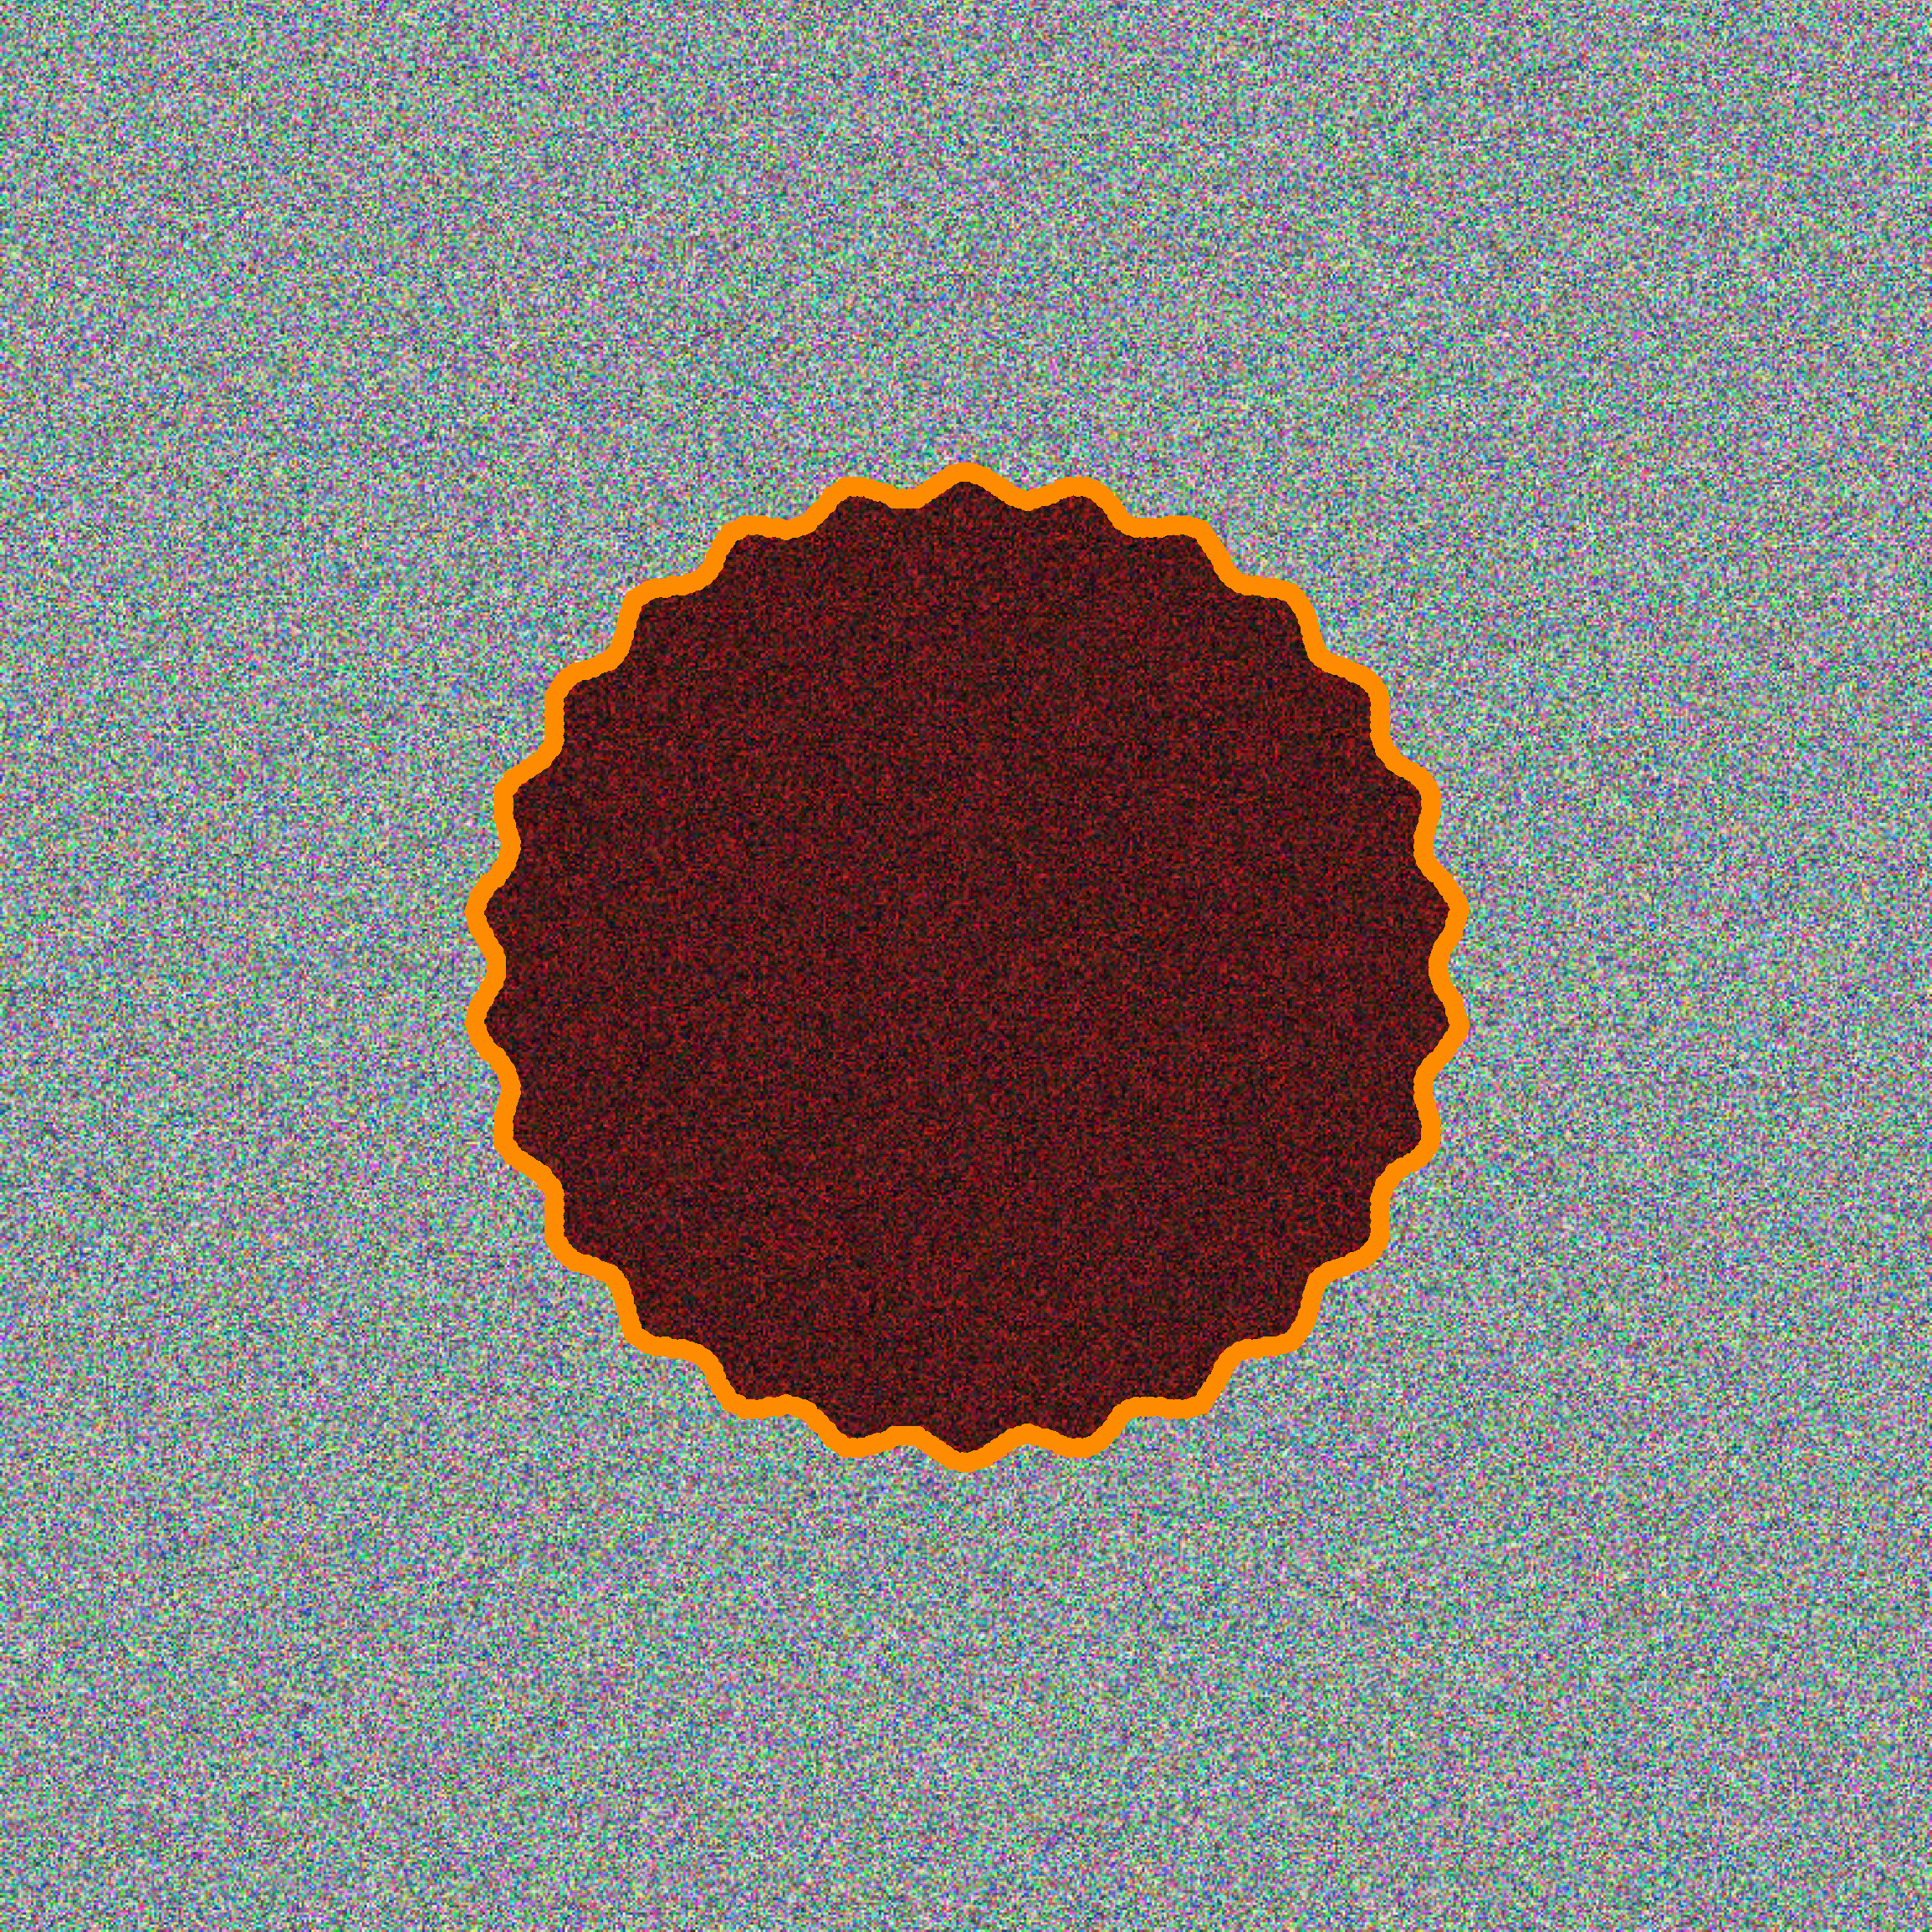
\includegraphics[width=0.3\linewidth]{GR_sim_image}
     }
    \\
     \subfloat[GR cropped to FLEV \label{GR_images:b}]{%
       \includegraphics[width=0.3\linewidth]{GT_flev_crop}
     }
     \subfloat[GR cropped to SF \label{GR_images:c}]{%
       \includegraphics[width=0.3\linewidth]{GT_sf_crop}
     }\\
     \subfloat[GR to S01 \label{GR_images:d}]{%
       \includegraphics[width=0.3\linewidth]{GR_sub_scene_07}
     }
     \subfloat[GR to S02 \label{GR_images:e}]{%
       \includegraphics[width=0.3\linewidth]{GR_sub_scene_10}
     }
    \caption{Ground references images overlain on the Pauli polarimetric color composite.}
     \label{GR_images} 
\end{figure}

The images in Fig.~\eqref{LA_GR_images} show the region in LA acquired with UAVSAR sensor on two different dates, April 2009 and May 2015.
\begin{figure}[ht!]
    \centering
     \subfloat[GR to LAA \label{LA_GR_images:a}]{%
       \includegraphics[width=0.25\textwidth]{GR_la_imag1_april_2009}
     }
     \subfloat[GR to LAM \label{LA_GR_images:b}]{%
       \includegraphics[width=0.25\linewidth]{GR_la_imag1_may_2015}
     }
    \caption{Ground references images overlain on the Pauli polarimetric color composite.}
     \label{LA_GR_images} 
\end{figure}



\subsection{The Gambini Algorithm (GA)}
The GA attempts to find evidence of an edge locally over a thin strip of PolSAR data. The thin strip of data is analyzed to find evidence of textural properties change. A border between regions with different characteristics along the strip is defined at the position of maximal change. The technique utilizes a ray-casting approach to search for the evidence of an edge by maximizing a value function. The proposed algorithm, initially, was computational expensive and achieved the detection of the borders by computing a likelihood function iteratively. \citet{EdgeDetectionDistancesEntropiesJSTARS} reduced the computational cost in the GA approach by using stochastic distance between the PolSAR samples. \citet{GeodesicDistanceGI0JSTARS} employed the geodesic distance between SAR  intensity samples in the GA as a measure of dissimilarity between the probability distribution models for feature extraction and region discrimination.  
The strength of the GA is demonstrated by its applicability under noisy (or speckled) conditions with any mathematical distribution model suitably fitting the PolSAR data. 
The mathematical models incorporate parameters to quantify areas with varying degrees of roughness, which essentially assists in demarcating regions with different textures.


\subsection{Distributions}
PolSAR systems register  the difference between the transmission and reception of amplitude and phase of backscattered,and  linear combinations, 
yielding four polarization channels:  $S_\text{HH}$, $S_\text{HV}$, $S_\text{VH}$, and $S_\text{VV}$  
(H for horizontal and V for vertical polarization).
%
If the reciprocity theorem conditions~\cite{MicrowaveRadarRadiometricRemoteSensing} are satisfied, then 
$S_\text{HV}=S_\text{VH}$.
%
Defining the single-look scattering vector as
\begin{equation}\label{vetor_lexicografico_3d}
\mathbf{S}=\left[
	\begin{array}{ccc}
	S_\text{HH}& S_\text{HV}& S_\text{VV}\\
\end{array}\right]^\text{T}.
\end{equation}
Thus, the scaled multilook PolSAR return has, in each pixel, the form:
$$
\bm{Z}
=
\frac{1}{L}
\sum_{\ell=1}^L
\begin{bmatrix}
S_{\text{HH}}^{(\ell)}\\
S_{\text{HV}}^{(\ell)}\\
S_{\text{VV}}^{(\ell)}
\end{bmatrix}
%
\begin{bmatrix}{S_{\text{HH}}^{*(\ell)}} &{S_{\text{HV}}^{*(\ell)}} &{S_{\text{VV}}^{*(\ell)}}
\end{bmatrix}
,
$$
where $L$ is the look number, and $S_i$ with $i\in \{\text{HH}, \text{HV}, \text{VV}\}$ is the scattering in each direction. The symbol * represents the complex conjugate.
%where F(ℓ)A,i∈\mathbbmCF_{\text{A},i}^{(\ell)}\in\mathbbm{C} is the scattering in channel A∈{H,V}\text{A}\in\{\text{H},\text{V}\} at the iith individual scatterer and ℓ\ell-th look. 

\citet{StatisticalAnalysisBasedonaCertainComplexGaussianDistributionanIntroduction}, in the context of Statistical Optics, discussed the properties of the full covariance matrix.
\citet{IntensityandPhaseStatisticsofMultilookPolarimetricandInterferometricSARImagery} derived several of its marginal distributions.
\citet{ATrivariateChiSquaredDistributionDerivedfromtheComplexWishartDistribution} obtained the joint distribution of the three intensity channels.

The Wishart distribution is the accepted model for data in covariance matrix format assuming fully developed speckle.
The reader is referred to the work by \citet{PolSARModelswithMultimodalIntensities} for details and extensions.
The Probability Density Function (PDF) that characterizes the Wishart distribution is
\begin{equation}\label{cap_acf_9}
    f_{\mathbf{Z}}(\mathbf{Z};\Sigma,L)=\frac{L^{mL}|\mathbf{Z}|^{L-m}}{|\Sigma|^{L}\Gamma_m(L)} \exp(-L\traco(\Sigma^{-1}\mathbf{Z})), \\
\end{equation}
where, $\traco(\cdot)$ is trace operator, $\Sigma$ is the covariance matrix,  $\Gamma_m(L)$ is the Gamma multivariate function defined by:
\begin{equation}\label{multi_gamma_func}
	\Gamma_m(L)=\pi^{\frac{1}{2}m(m-1)} \prod_{i=0}^{m-1}\Gamma(L-i) \\
\end{equation}
and $\Gamma(\cdot)$ is the gamma function. 

The Wishart distribution works with fully polarimetric information. We work with intensity (amplitude) information. In the equations from \eqref{eq:pdfGammaUniv} to \eqref{eq:LogLikelihoodGamma_red_span}, we describe physical probability density distributions using the intensity information and its log-likelihood reduced function.

\begin{enumerate}[leftmargin=*,labelsep=4.9mm]
\item Gamma univariate PDF to intensities: We assume that the distribution of each intensity channel is a Gamma law with probability density function
\begin{equation}
f_{\mathbf{Z}}(z;\mu,L)=\frac{L^{L}}{\Gamma(L)\mu^{L}} z^{L-1}\exp\left\{-\frac{L}{\mu}z\right\},
\label{eq:pdfGammaUniv}
\end{equation}
where $L>0$ (rather than $L\geq 1$ to allow for flexibility), and $\mu>0$ is the mean. 	  
Given the sample $\bm z = (z_1,\dots,z_n)$ obtained from SAR/PolSAR images, the reduced log-likelihood of this model is
\begin{equation}
\ell(\bm z; L,\mu) = n \big[L\ln (L / \mu) - \ln \Gamma(L)\big]+L \sum_{k=1}^{n}\ln z_k -\frac{L}{\mu}\sum_{k=1}^{n}z_k.
\label{eq:LogLikelihoodGamma_2_param}
\end{equation}
%\item Probability Density Function Bivariate Product of the Intensities:
%We can look up this probability density function bivariate in the
%reference~\citet{IntensityandPhaseStatisticsofMultilookPolarimetricandInterferometricSARImagery}
% AAB This equation is larger than the page.
%\begin{equation}
%	f(z_1,z_2;\rho,L, \Sigma_{11}, \Sigma_{22})=\frac{L^{L+1}\left(z_1z_2\right)^{\frac{L-1}{2}}\exp\left(-\frac{L\left(\frac{z_1}{\Sigma_{11}}+\frac{z_2}{\Sigma_{22}}\right)}{1-|\rho|^2}\right)}{(\Sigma_{11}\Sigma_{22})^{\frac{L+1}{2}}\Gamma(L)(1-|\rho|^2)|\rho|^{L-1}}I_{L-1}\left(2L\sqrt{\frac{z_1z_2}{\Sigma_{11}\Sigma_{22}}}\frac{|\rho|}{1-|\rho|^2}\right).
% \label{eq:func_biv_prod_inten_z1_z2}
%\end{equation}
%
%We deduce the reduced form from equation~\eqref{eq:func_biv_prod_inten_z1_z2}
%\begin{equation}
%\begin{split}
%\ell(\bm z_1, \bm z_2;\rho, L, \Sigma_{11}, \Sigma_{22})&=n\left[(L+1)\ln L - \ln\Gamma(L)- \ln(1-|\rho|^2)-(L-1)\ln|\rho|\right. \\
%	                    &-\left.\frac{L+1}{2}\ln\Sigma_{11}-\frac{L+1}{2}\ln\Sigma_{22}\right] \\
%                        &+\frac{L}{2}\sum_{k=1}^{n} \ln z^1_k +\frac{L}{2} \sum_{k=1}^{n}\ln z^2_k\\
%                        &-\frac{L}{\Sigma_{11}(1-|\rho|^2)}\sum_{k=1}^{n}z^1_k-\frac{L}{\Sigma_{22}(1-|\rho|^2)}\sum_{k=1}^{n}z^2_k\\
%	&+\sum_{k=1}^{n}\ln I_{L-1}\left(2L\sqrt{\frac{z^1_kz^2_k}{\Sigma_{11}\Sigma_{22}}}\frac{|\rho|}{1-|\rho|^2}\right)
%\end{split}
% \label{eq:log_vero_biv_prod_red}
%\end{equation}
\item PDF ratio of intensities: The density that characterizes the ratio of any pair of intensities is
\begin{equation}
	f(\mu;\rho,L)=\frac{\Gamma(2L)(1-|\rho|^2)^{L}(1+\mu)\mu^{L-1}}{\Gamma(L)\Gamma(L)\left[(1+\mu)^2-4|\rho|^2 \mu \right]^{\frac{2L+1}{2}}},
\label{eq:pdf_ratio_intensities}
\end{equation}
where, $\rho>0$ and $L>0$. We can normalize the ratio of intensities as: 
\begin{equation}
 \mu=\frac{\sum_{k=1}^{n}\frac{|S_i(k)|^2}{\Sigma_i}}{\sum_{k=1}^{n}\frac{|S_j(k)|^2}{\Sigma_j}}=\frac{\sum_{k=1}^{n}|S_i(k)|^2}{\tau\sum_{k=1}^{n}|S_j(k)|^2},\\
 \label{eq:ratio_intensities_norm}
\end{equation}
where $\tau=\frac{\Sigma_i}{\Sigma_j}$ with $i\in \{\text{HH}, \text{HV}, \text{VV}\}$ and $i \neq j$. If we define $z=\tau \mu$ and verify that the variable change in equation \eqref{eq:pdf_ratio_intensities}, we obtain: 
\begin{equation}
	f(z;\rho,L,\tau)=\frac{\tau^L\Gamma(2L)(1-|\rho|^2)^{L}(\tau+z)z^{L-1}}{\Gamma(L)\Gamma(L)\left[(\tau+z)^2-4\tau|\rho|^2z \right]^{\frac{2L+1}{2}}}.\\
 \label{eq:pdf_ratio_intensities_tau_z}
\end{equation}

Given the sample $\bm z = (z_1,\dots,z_n)$ obtained from SAR/PolSAR images, we deduce the log-likelihood function in your reduced format
\begin{equation}
\begin{split}
    \ell(\bm z;\rho, L, \tau)&=n\left(L\ln\tau +\ln\Gamma(2L)+L\ln(1-|\rho|^2)-2\ln\Gamma(L)\right)\\
                         &+\sum_{k=1}^{n}\ln(\tau+z_k)+L\sum_{k=1}^{n}\ln z_k-\frac{2L+1}{2}\sum_{k=1}^{n} \ln\left[(\tau+z_k)^2-4\tau|\rho|^2z_k\right]\\
\end{split}
\label{eq:log_like_ratio_intensidade_red_tau_z}
 \end{equation} 
%
%\item Product of the intensities: The probability density univariate magnitude of the product
%\begin{equation}
%	f_{Z}(z;\rho, L)=\frac{4L^{L+1} z^L}{\Gamma(L)(1-|\rho|^2)}I_0\left(\frac{2|\rho|L z}{1-|\rho|^2}\right)K_{L-1}\left(\frac{2L z}{1-|%\rho|^2}\right),
% \label{eq:pdf_mag_prod}
%\end{equation}
%where $I_0$ e $K_{L-1}$ are modified Bessel functions, with $\rho>0$, and $L>0$.
%
%The reduced log-likelihood function is, thus:
%\begin{equation}
%\begin{split}
%    \ell(z;\rho, L)&=n\left[(L+1)\ln L-\ln\Gamma(L)-\ln(1-|\rho|^2)\right]\\
%                         &+L\sum_{k=1}^{n} \ln z_k+\sum_{k=1}^{n}\ln I_0\left(\frac{2|\rho|L z_k}{1-|\rho|^2}\right)+ \sum_{k=1}^{n}\ln %K_{L-1}\left(\frac{2L z_k}{1-|\rho|^2}\right).
%\end{split}
%\label{eq:eq_log_vero_mag_prod_red}
% \end{equation}
% %
% \item Trivariate Multilook Intensities 
 
\item PDF to Span -
Ref~\cite{fwzjn} shows that we can use a Gamma distribution to model the \textit{span} by considering
\begin{equation}
	f_{\mathbf{S}}(s;\mu,L)=\frac{L^{L}}{\Gamma(L)\mu^{L}} s^{L-1}\exp\left\{-\frac{L}{\mu}s\right\},
 \label{eq:gamma_span}
\end{equation}
where, $\mu>0$, $L>0$, e $s$ is the element of the set \textit{span}($\mathbf{S}$).

For the probability density function~\eqref{eq:gamma_span}, and the sample $\bm s = (s_1,\dots,s_n)$ extract to SAR/PolSAR, we obtain the log-likelihood reduced function
\begin{equation}
\ell(\bm s;\mu, L) = 
n \left[L\ln \frac{L}{\mu} - \ln \Gamma(L)\right]
+L \sum_{k=1}^{n}\ln s_k -\frac{L}{\mu}\sum_{k=1}^{n} s_k.
\label{eq:LogLikelihoodGamma_red_span}
\end{equation}
\end{enumerate}
%

We obtain the parameters for the maximum likelihood estimator (MLE) by maximizing the reduced log-likelihood function with the Broyden-Fletcher-Goldfarb-Shanno (BFGS) method~\cite{ht}.

After finding the parameters, we built the log-likelihood total to find the edge evidence by applying the Generalized Simulated Annealing (GenSA)~\cite{xgsh} method. 

The log-likelihood total is non-differentiable and shows oscillation at the extremities of its domain. The GenSA solves the first problem. The second problem was solved by defining a slack constant to domain extremities. For more details see~\citet{FusionofEvidencesinIntensitiesChannelsforEdgeDetectioninPolSARImages}.
%
\subsection{Information Fusion Methods}
Ref~\cite{FusionofEvidencesinIntensitiesChannelsforEdgeDetectioninPolSARImages} proposes information fusion of the detected edge evidence in each intensity channel of a PolSAR image. Based on these ideas, we propose inserting the channel obtained with a PDF ratio of intensities and PDF to \textit{span}. We use the principal components analysis (PCA) method because, besides being considered an information fusion method of the evidence of edges to the channels, it can indicate the weighting of each channel to be highlighted or discarded in the information fusion.

The channels highlighted in the weighting will be used in the statistic receiver operating characteristic (S--ROC) information fusion method proposed in Ref~\cite{gs}, we named the information fusion of the threshold S-ROC ($\tau$S-ROC). Below, we discuss more details of PCA, S-ROC, and $\tau$S-ROC methods.

For Fusion methods, we assume we have $n_c$ binary images $\{\widehat{\bm\jmath}_c\}_{1\leq c\leq n_c}$ in which~$1$ denotes an estimate of edge and $0$ otherwise.
They have a common size $m\times n$; denote $\ell=mn$.
These images will be fused to obtain the binary image $\bm I_F$.
%
\subsubsection{PCA Fusion Methods}
The method PCA Fusion is based on~\cite{n_r,mit} and comprised of the following steps:
\begin{enumerate}[label=(\roman*)]
\item Stack the binary images $\bm{\widehat\jmath}_c$ in column vectors to obtain the matrix $\bm X_{\ell\times n_c}$.\label{item:PCA_1}
\item Calculate the covariance matrix $\bm C_{n_c\times n_c}$ of $\bm X_{\ell\times n_c}$.\label{item:PCA_2}
\item Compute the eigenvalues ($\bm\Lambda$) and corresponding eigenvectors ($\bm V$) of the covariance matrix. Sort the eigenvalues and corresponding eigenvectors in decreasing order. \label{item:PCA_3}
\item Compute the vector $\bm P=(P(1),\dots,P(n_c))=(\sum_{c=1}^{n_c} V(c))^{-1}{\bm V}$, where $\bm V$ is the eigenvector associated with the highest eigenvalue of $\bm C_{n_c\times n_c}$; notice that $\sum_{c=1}^{n_c} P(c)=1$. \label{item:PCA_4}
\end{enumerate}
 
The PCA method indicates the coefficients $P(\cdot)$ providing the weighting to each channel with the edge evidences involved on fusion of information. This weighting shows the channel's importance in the edge evidences' fusion process; therefore, we can choose a setting to use in $\tau$S-ROC fusion.
%
\subsubsection{S--ROC and \texorpdfstring{$\tau$S}--ROC Fusion Methods}
The S--ROC was proposed and described on~\cite{gs}. We propose a modification for this method described below:
\begin{enumerate}[label=(\roman*)]  
\item Add the binary images $\bm{\widehat\jmath}_c$ to produce the frequency matrix ($\bm V$).\label{item:eROC_1}
\item Use automatics optimal thresholds ranging from $t=1,\dots,n_c$ on $\bm V$ to generate matrices $\bm M_t$.\label{item:eROC_2}
\item Compare each $\bm M_t$ with all $\bm{\widehat\jmath}_c$, find the confusion matrix to generate the ROC curve. 
The optimal threshold corresponds to the point of the ROC curve closest (in the sense of the Euclidean distance) to the diagnostic line. \label{item:eROC_3}
\item Use PCA information to choose the channels to fusion. We compare each PCA coefficient with a threshold ($\tau$) defined empirically if coefficients great than $\tau$ storage to use in S--ROC. For this article, the threshold used was 10\% of the sum of the PCA coefficients. Furthermore, we named these methods by $\tau$S--ROC.    
\item The fusion $\bm I_F$ is the matrix $\bm M_t$ which corresponds to the optimal threshold.\label{item:eROC_4}
\end{enumerate}
%
\subsection{Measures of Quality}
We used the Hausdorff distance (Hd) as a measure to quantify the performance of the edge evidences estimates, edges S--ROC and $\tau$S--ROC fusion. The metric Hausdorff is defined as Hd = $\max_{p\in P}\min_{p^{'}\in P^{'}}\vert\vert p-p^{'}\vert\vert$, where P and $\text{P}^{'}$ represent the points in the true edge (Ground Reference - GR) and points obtained by the methodology proposal in this article. The smaller the Hd value the better the edge. For more details see~\citep{taha_hanb} and~\citep{rey_sar_frery_del}. 
%
\section{Results}\label{sec:Results}
We run the experiments presented in this work with a computer running Intel\copyright\ Core i7-9750HQ CPU 
\SI{2.6}{\giga\hertz}, \SI{16}{\giga\byte} of RAM memory.
 %
 \subsection{Flower simulated image}
For the Flower with dimension $800 \times 800$ pixels, we defined the slack constant as 10 pixels, the radial number is 100, and each radial has 300 pixels. The image has four nominal looks and nine channels.

Using the distribution ratio of intensities, we have pixel to pixel ratio for two channels. This fact could be a problem when creating an image because of divisions by zeros. However, to the Flower, this problem has yet to happen, which is different from the PolSAR image. Fig~\eqref{SimRatioRoi01_gray_HHVV_VVHH} shows the image ratio intensities HH/VV~\eqref{SimRatioRoi01_gray_HHVV_VVHH:a} and VV/HH~\eqref{SimRatioRoi01_gray_HHVV_VVHH:b} they present the ratio intensities image.  
\begin{figure}[hbt]
	\centering
     \subfloat[Channel HH/VV \label{SimRatioRoi01_gray_HHVV_VVHH:a}]{%
       \includegraphics[width=0.30\linewidth]{SimRatioHHVVRoi01_gray}
     }
     \subfloat[Channel VV/HH \label{SimRatioRoi01_gray_HHVV_VVHH:b}]{%
       \includegraphics[width=0.30\linewidth]{SimRatioVVHHRoi01_gray}
     }
     \caption{The worst ratio intensities SIM} 
     \label{SimRatioRoi01_gray_HHVV_VVHH} 
\end{figure}
%

Fig.~\eqref{sim_ev_intensities_and_ratio}  shows the intensity channel HH~\eqref{sim_ev_intensities_and_ratio:a} and span channel~\eqref{sim_ev_intensities_and_ratio:b} both have an excellent performance to detect edge evidence. Furthermore, Figs.~\eqref{sim_ev_intensities_and_ratio:c} and~\eqref{sim_ev_intensities_and_ratio:d} show a weak performance to detect edge evidence using the PDF ratio of intensities.
\begin{figure}[hbt]
	\centering
     \subfloat[Channel HH \label{sim_ev_intensities_and_ratio:a}]{%
       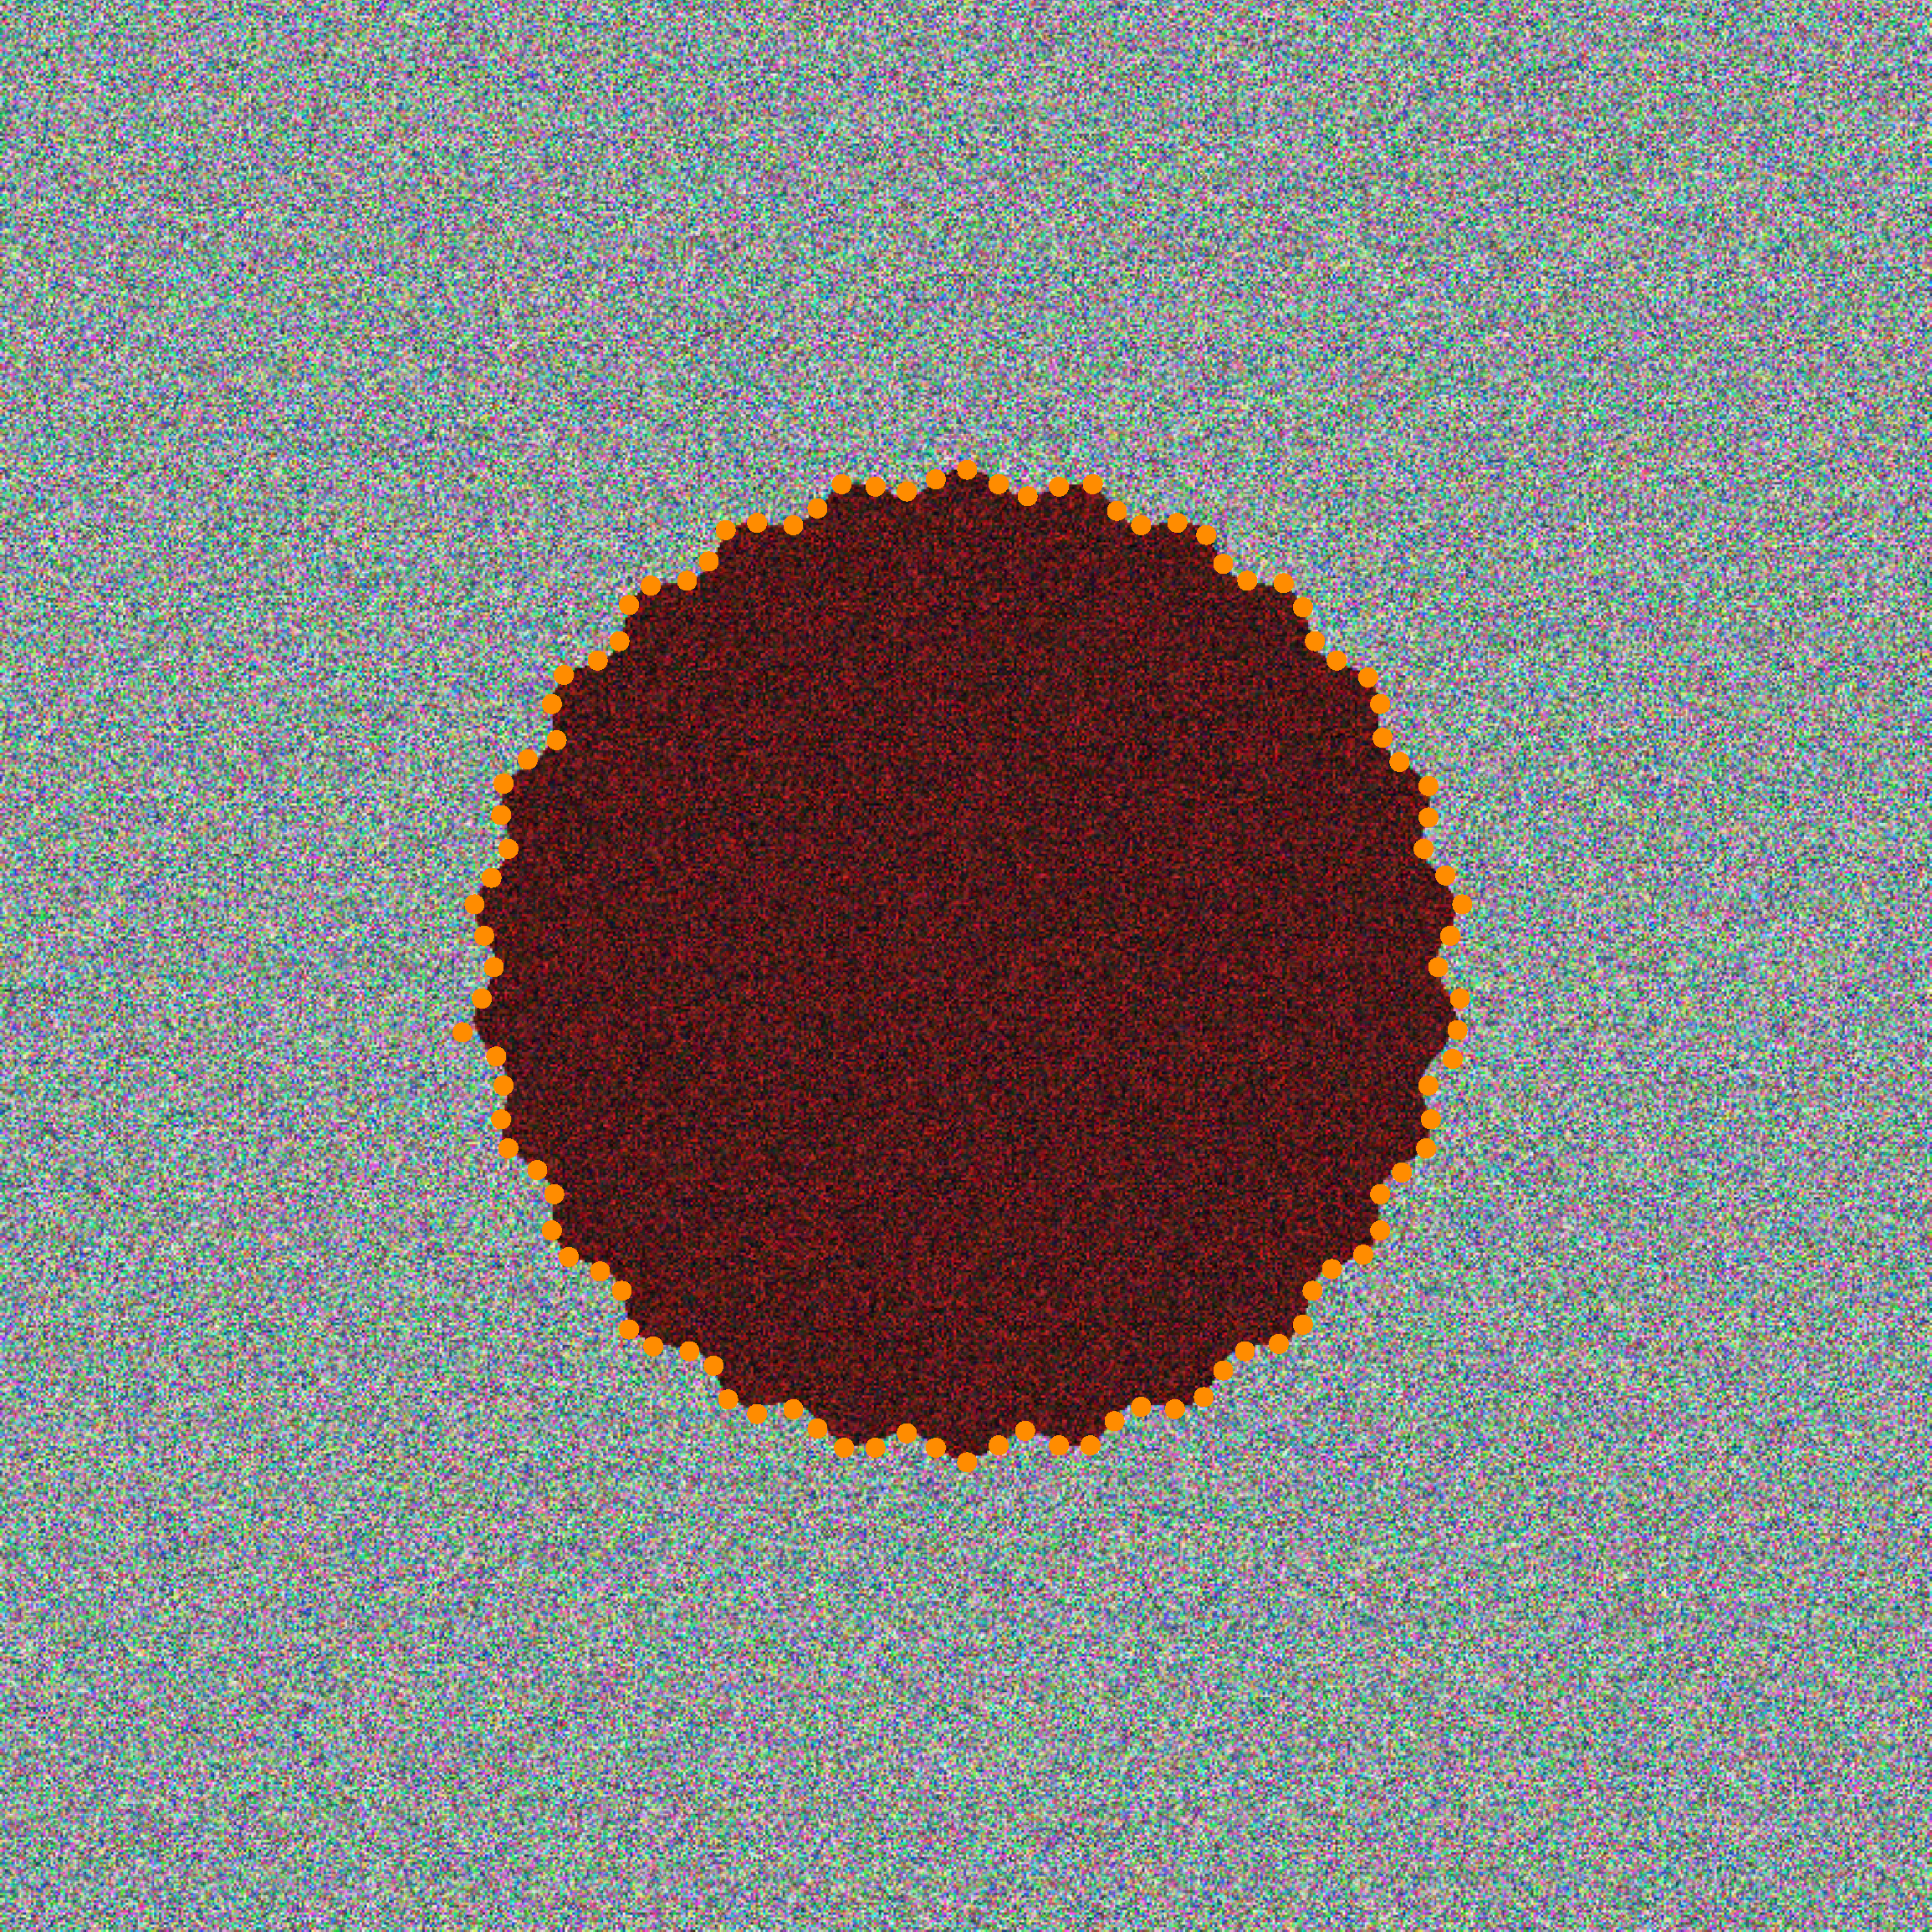
\includegraphics[width=0.25\textwidth]{SimEvChhRoi01}
     }
     \subfloat[Channel span \label{sim_ev_intensities_and_ratio:b}]{%
       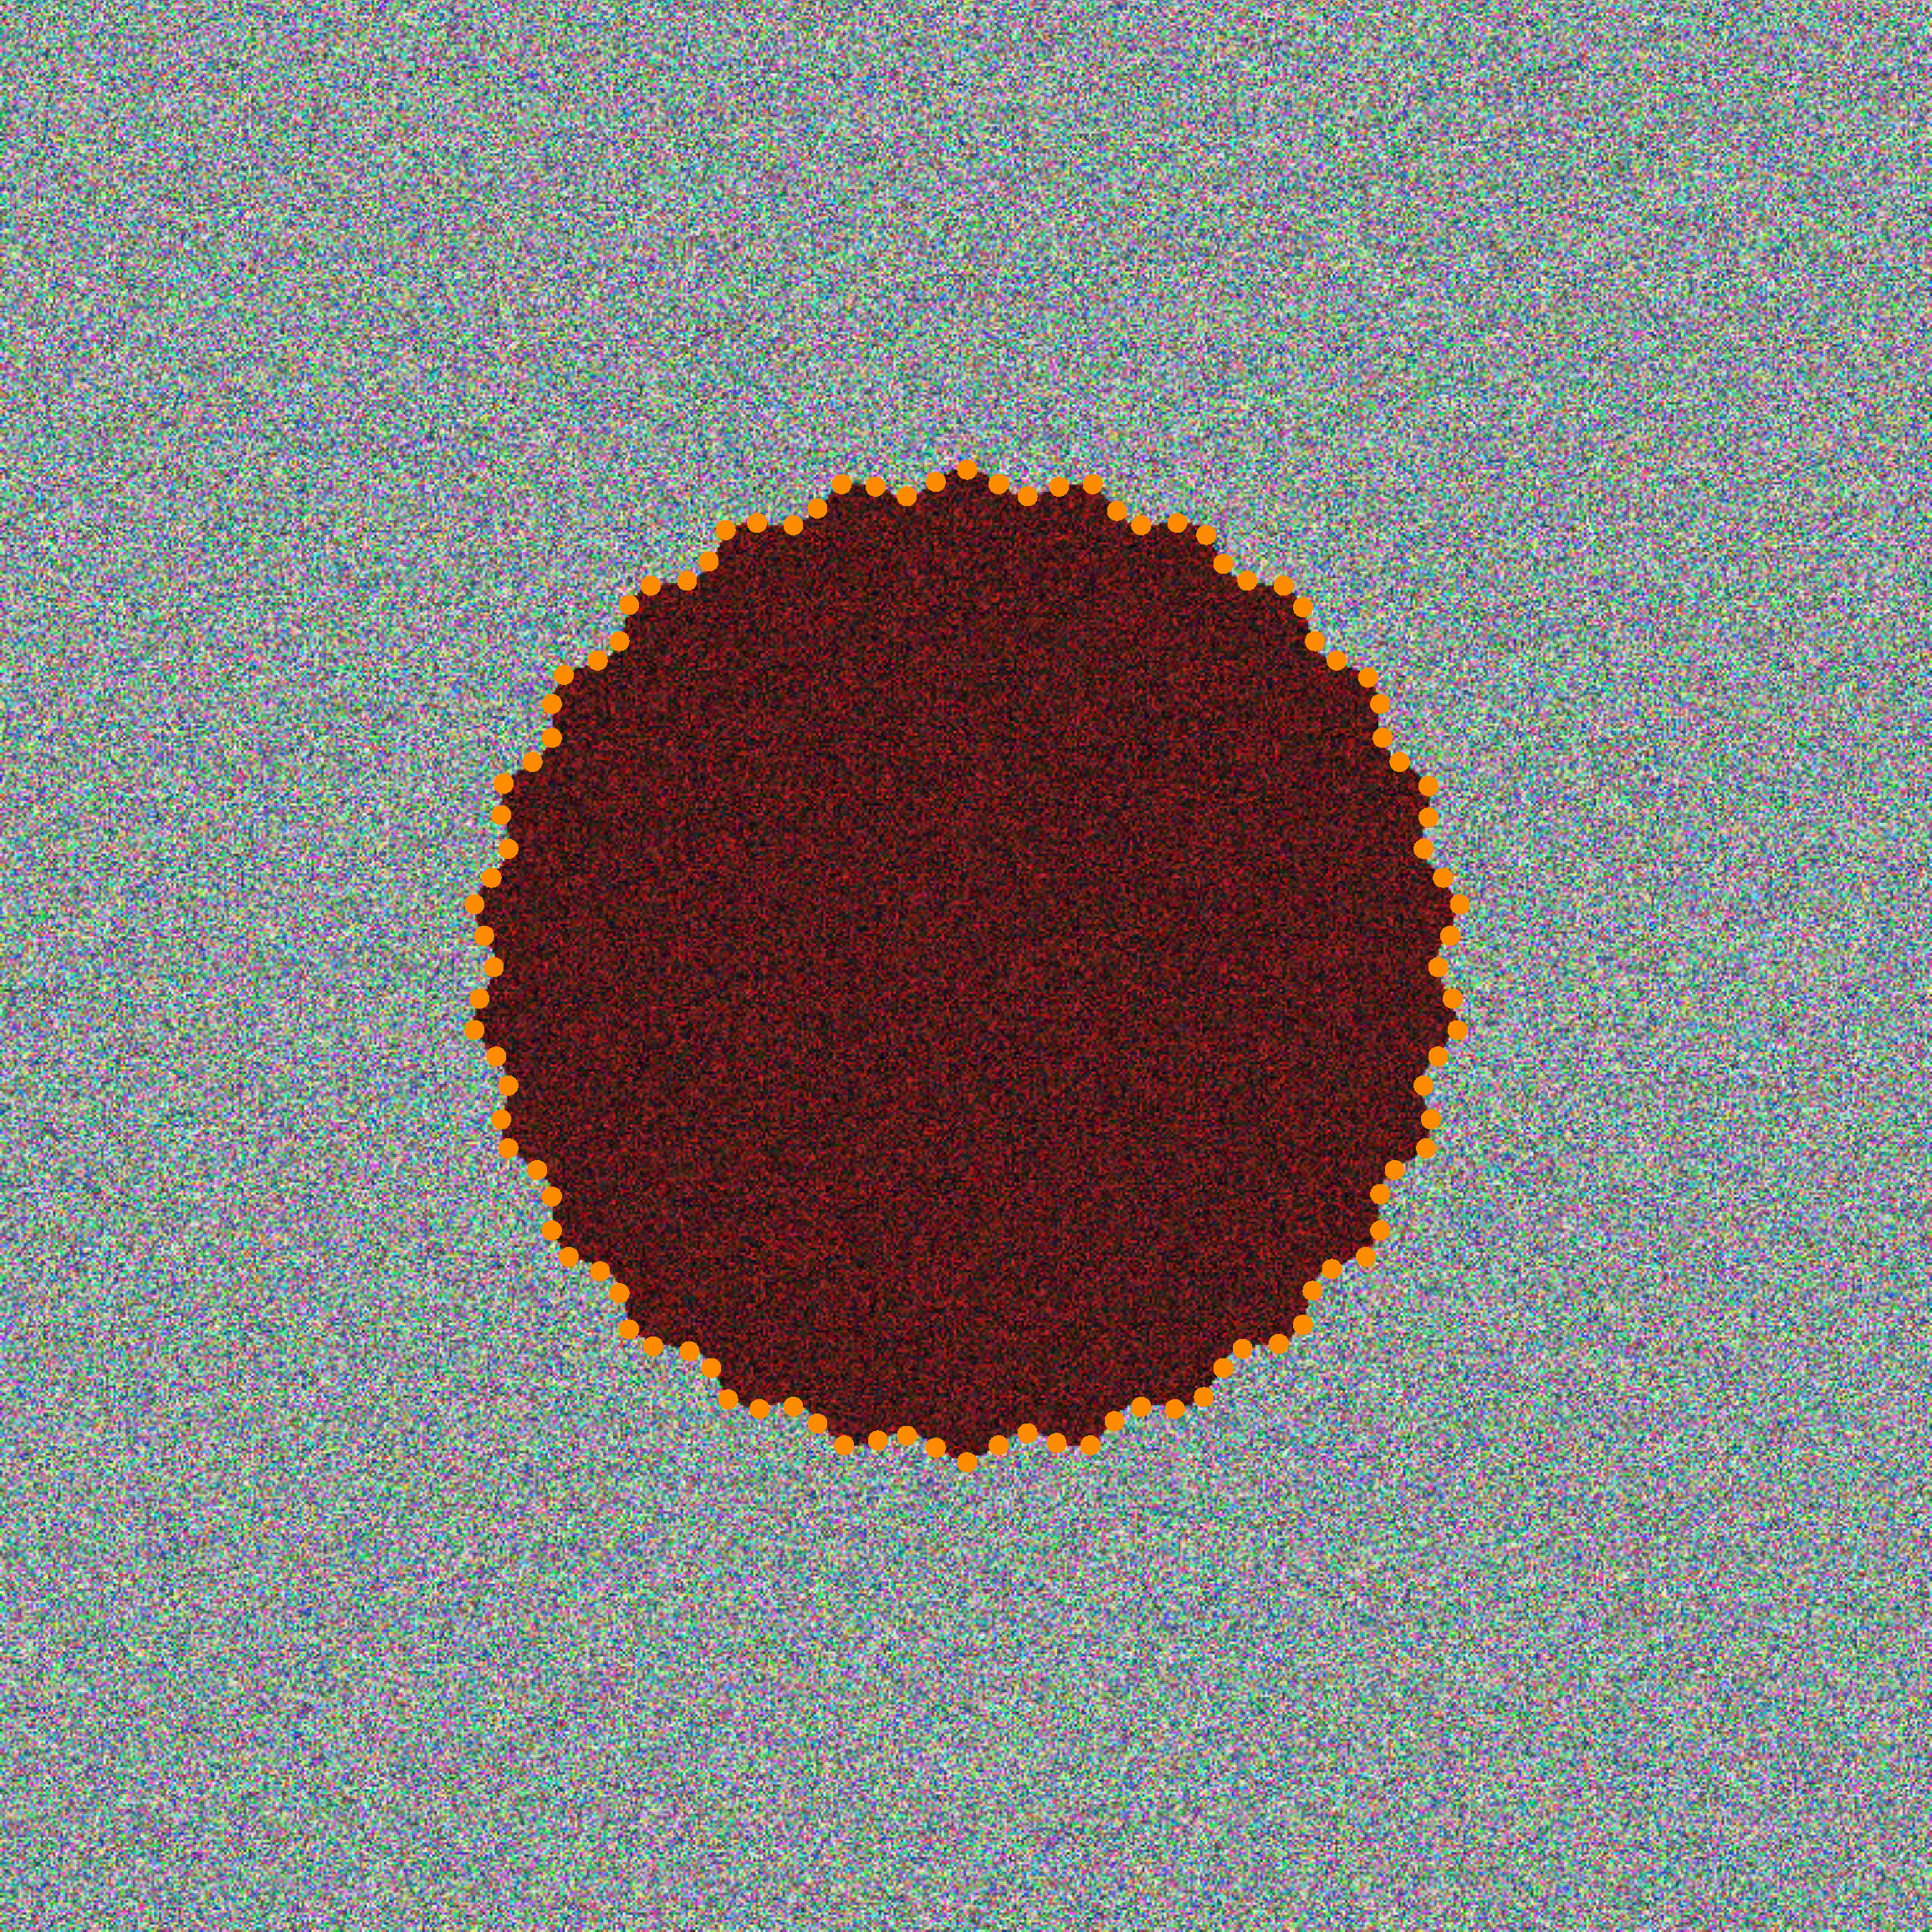
\includegraphics[width=0.25\linewidth]{SimEvSpanRoi01}
     }
     \subfloat[Channel HH/VV\label{sim_ev_intensities_and_ratio:c}]{%
       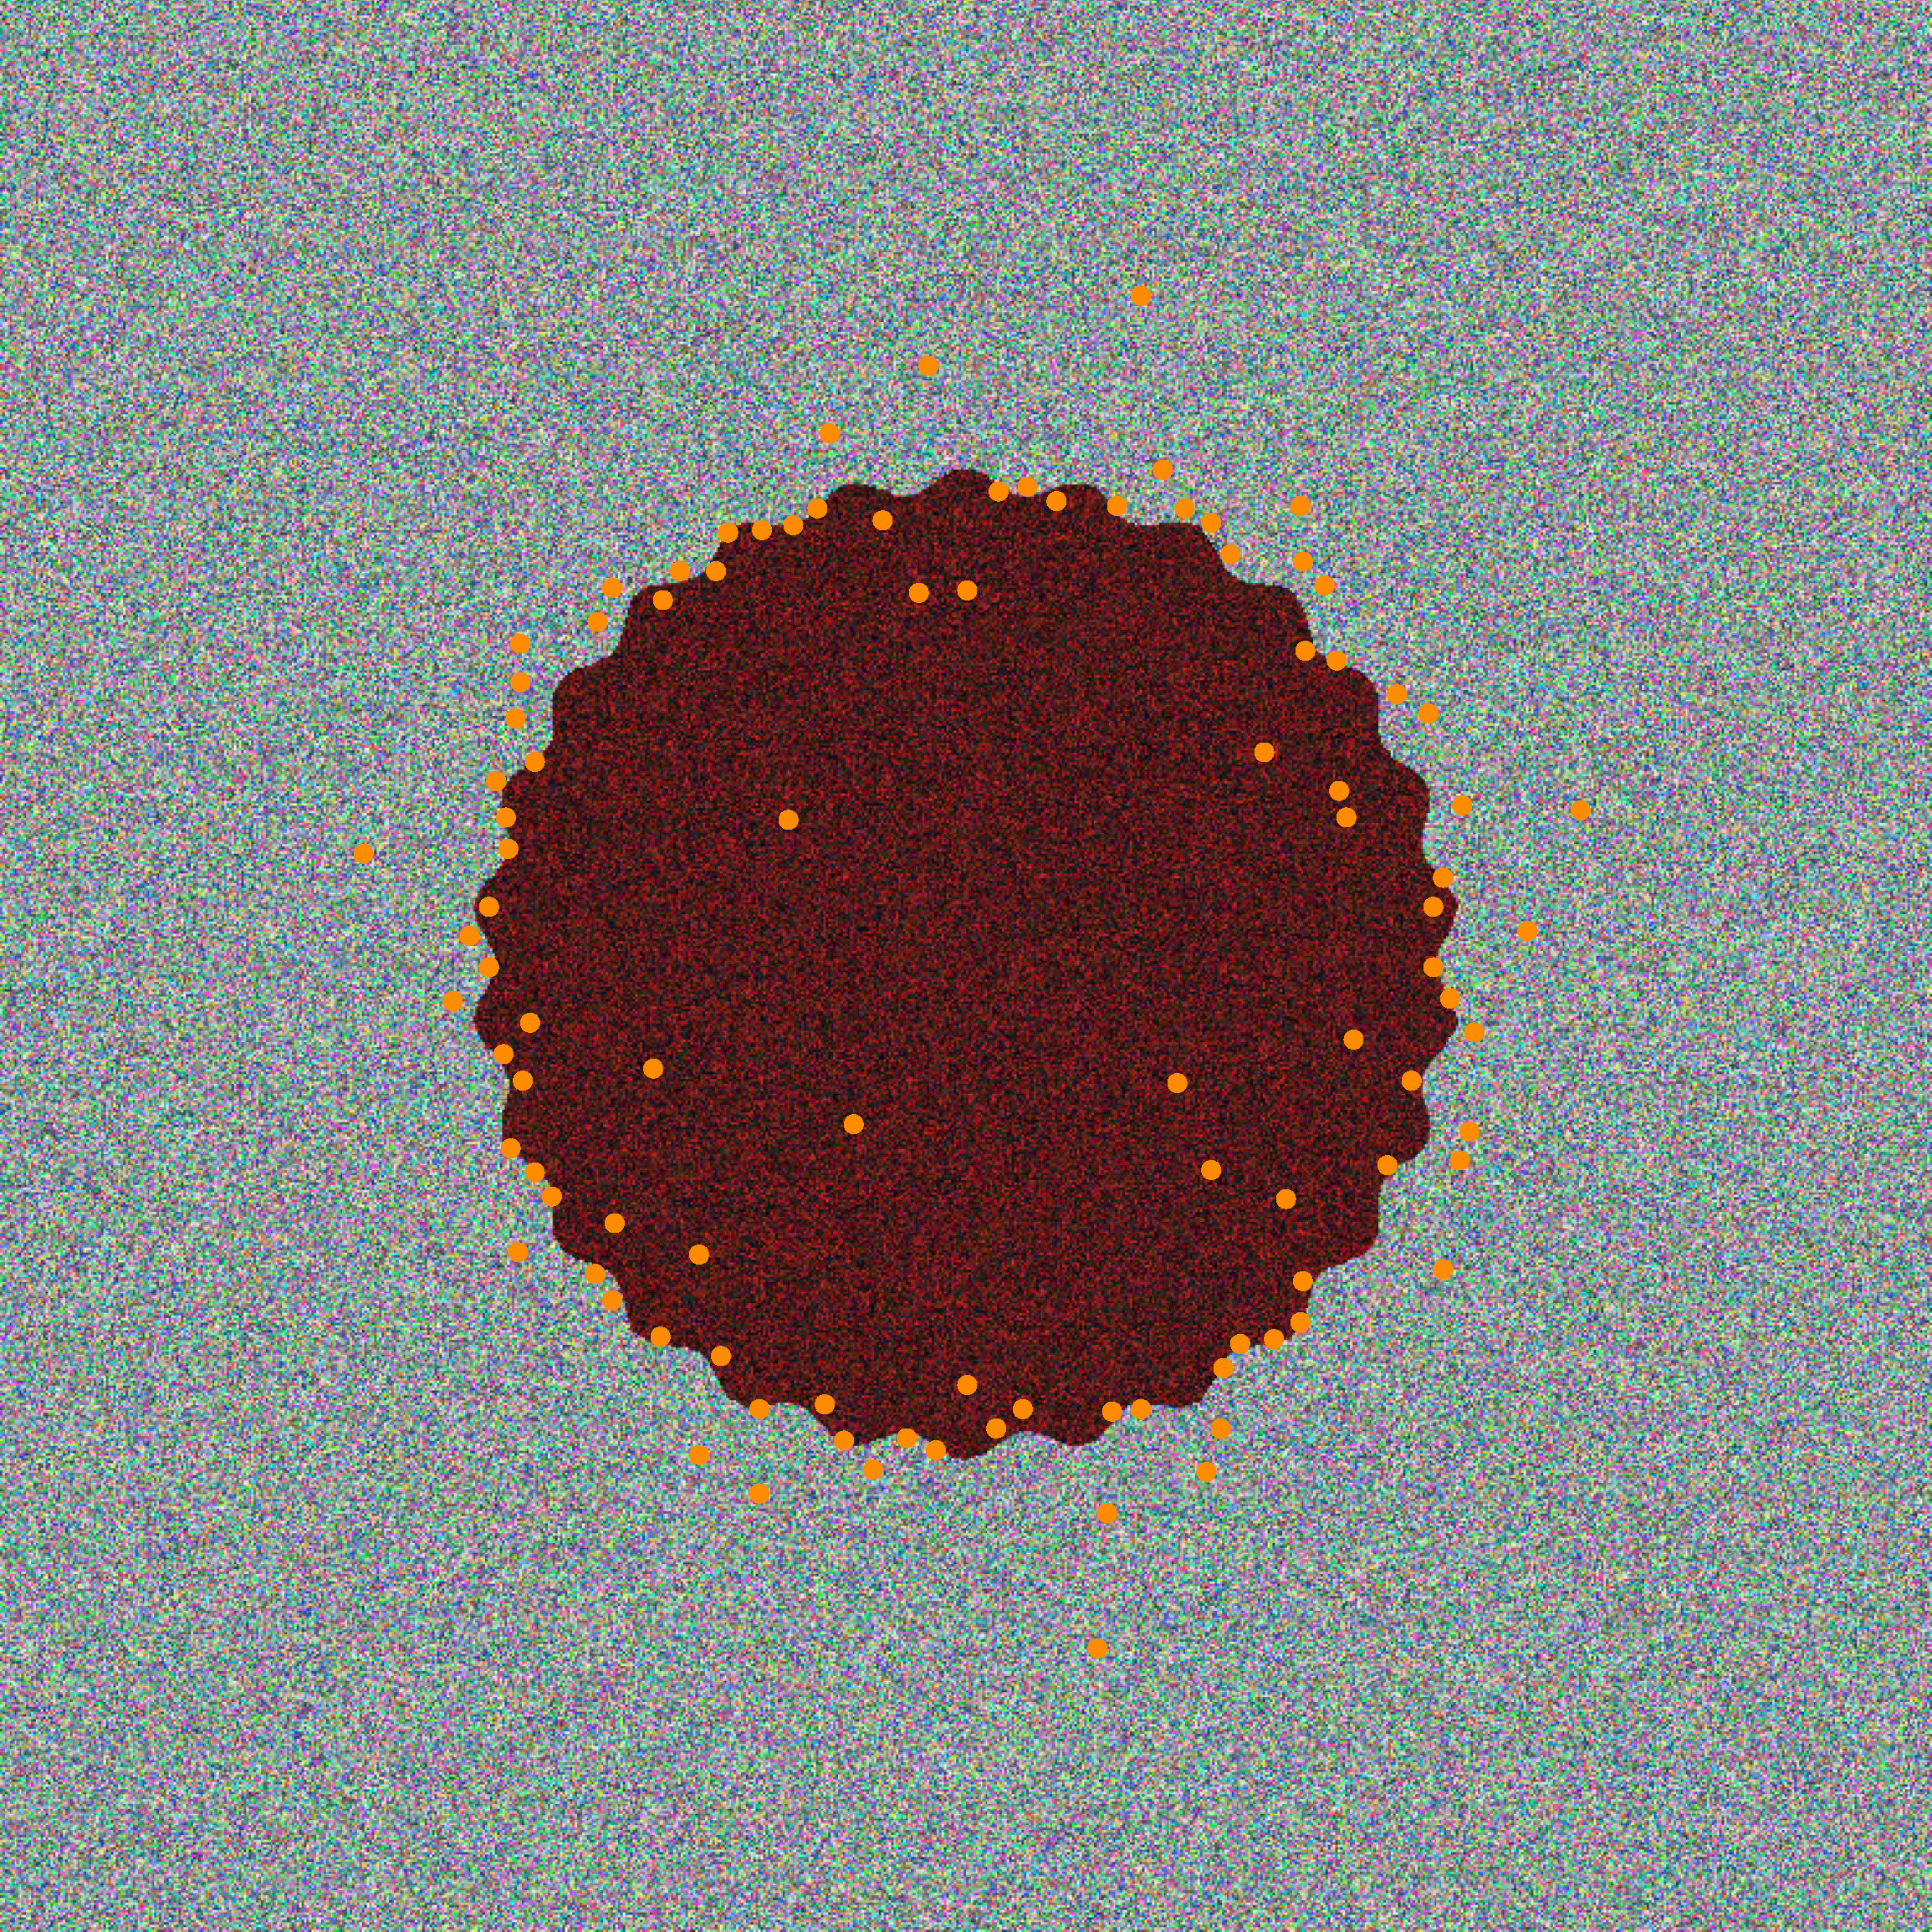
\includegraphics[width=0.25\linewidth]{SimEvRatioHHVVRoi01}
     }
    \subfloat[Channel VV/HH \label{sim_ev_intensities_and_ratio:d}]{%
       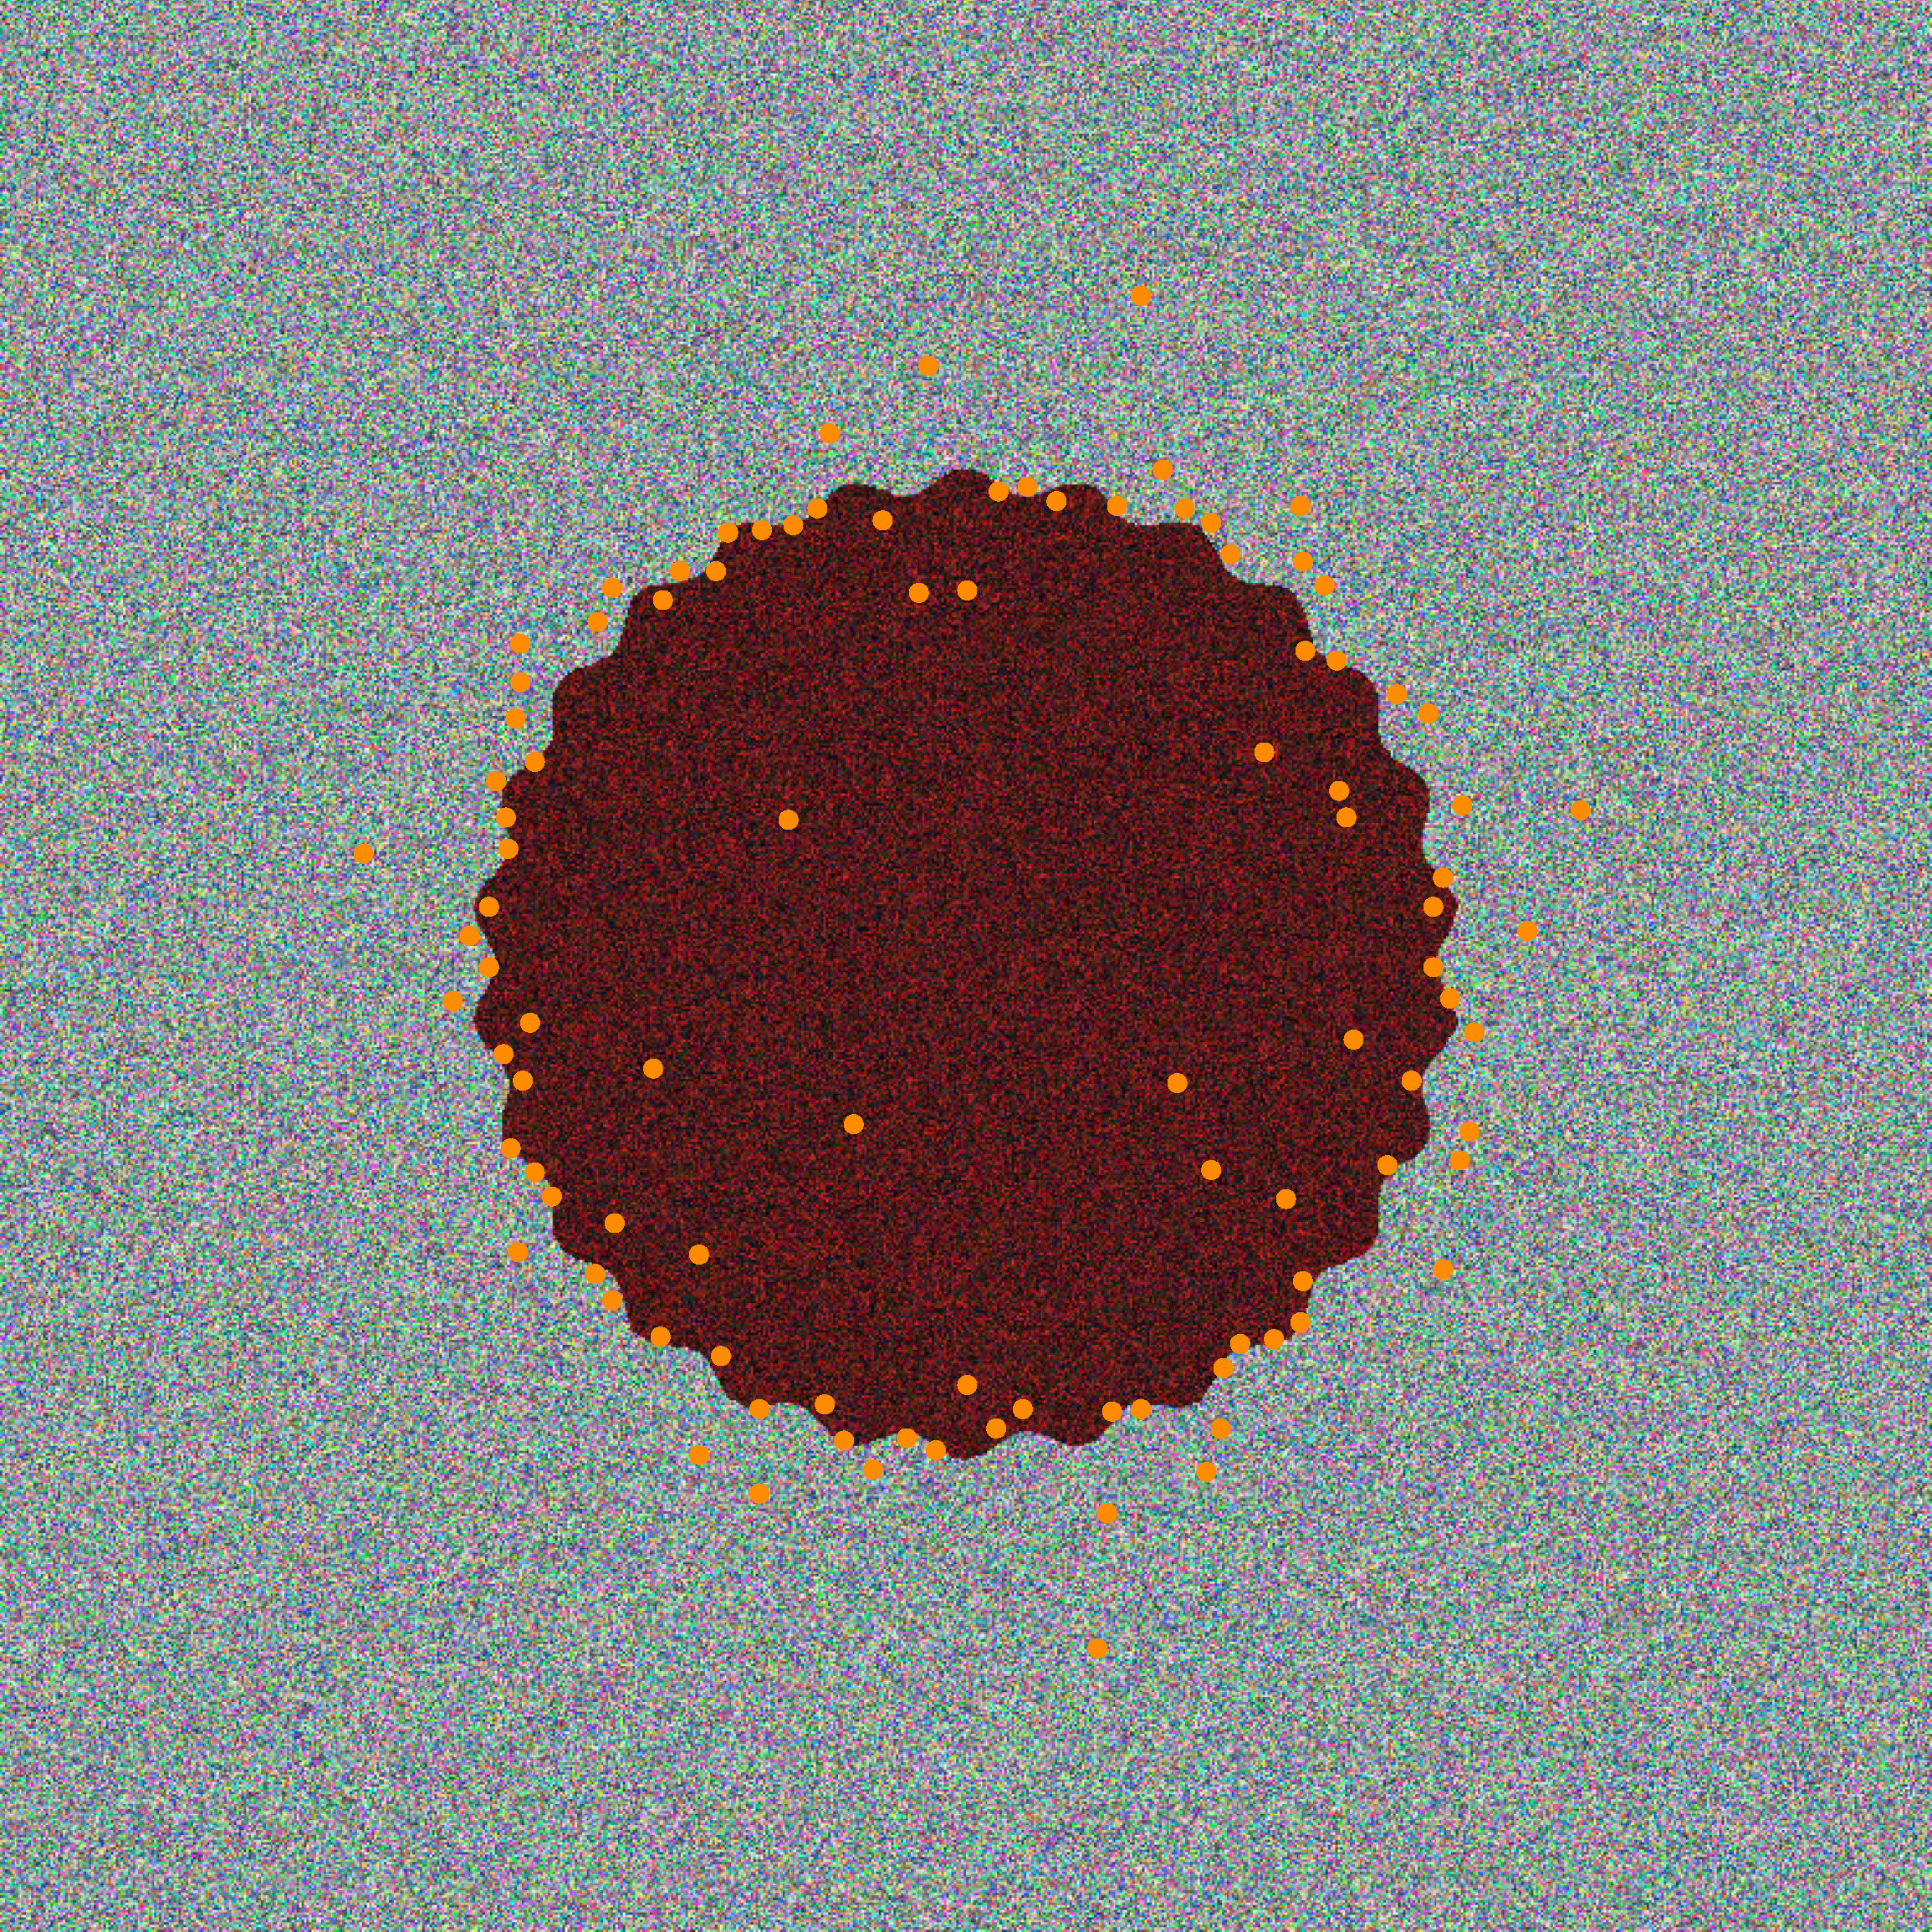
\includegraphics[width=0.25\linewidth]{SimEvRatioVVHHRoi01}
     }
     \caption{Edges evidences to four channel overlain on the Pauli polarimetric color composite.}
     \label{sim_ev_intensities_and_ratio} 
\end{figure}
 %%%%%%%%%
\subsection{Flevoland Images} 
The FLEV image has dimension $750\times 1024$ pixels, it is a PolSAR image captured by the airborne AIRSAR sensor with L-band. The image has four nominal looks and nine channels. 

For this image, we defined the slack constant as 15 pixels, the radial number is 100, and each radial has 120 pixels. If radial has pixels with value zero, then we remove these pixels.  

Using the distribution ratio of intensities, we have pixel to pixel ratio for two channels. Again, this fact is a problem when creating an image because of divisions by zero. Fig~\eqref{FlevRatioRoi01_gray_HHVV_VVHH} shows the ratio intensities image.   
\begin{figure}[hbt]
	\centering
     \subfloat[Channel HH/VV \label{FlevRatioRoi01_gray_HHVV_VVHH:a}]{%
       \includegraphics[width=0.30\linewidth]{FlevRatioHHVVRoi01_gray}
     }
     \subfloat[Channel VV/HH \label{FlevRatioRoi01_gray_HVHH_VVHH:b}]{%
       \includegraphics[width=0.30\linewidth]{FlevRatioVVHHRoi01_gray}
     }\\
     \caption{Ratio intensities images to Flevoland}
     \label{FlevRatioRoi01_gray_HHVV_VVHH} 
   \end{figure}
%

Fig~\eqref{flev_ev_hh_hv_vv} shows the methodology built with univariate gamma distribution and ratio distribution applied to  intensity channels.

Fig.~\eqref{flev_ev_hh_hv_vv}  shows the intensity channel HH~\eqref{flev_ev_hh_hv_vv:a} and span channel~\eqref{flev_ev_hh_hv_vv:b} both have an excellent performance to detect edge evidence. Furthermore, Figs.~\eqref{flev_ev_hh_hv_vv:c} and~\eqref{flev_ev_hh_hv_vv:d} show a weak performance to detect edge evidence using the pdf ratio of intensities.
  \begin{figure}[hbt]
	\centering
     \subfloat[Channel HH \label{flev_ev_hh_hv_vv:a}]{%
       \includegraphics[width=0.25\textwidth]{FlevEvChhRoi01_crop}
     }
     \subfloat[Channel Span \label{flev_ev_hh_hv_vv:b}]{%
       \includegraphics[width=0.25\linewidth]{FlevEvSpanRoi01_crop}
     }
     \subfloat[Channel HH/VV \label{flev_ev_hh_hv_vv:c}]{%
       \includegraphics[width=0.25\linewidth]{FlevEvRatioHHVVRoi01_crop}
     }
     \subfloat[Channel VV/HH\label{flev_ev_hh_hv_vv:d}]{%
       \includegraphics[width=0.25\linewidth]{FlevEvRatioVVHHRoi01_crop}
     }
     \caption{Edges evidences from the three intensity channels overlain on polarimetric color composite.}
     \label{flev_ev_hh_hv_vv} 
   \end{figure}
%%%%%%%%%%%%%%%%%%%%%%%%%%%%%%
\subsection{San Francisco Image} 
The San Francisco Bay image has dimension $450\times600$ pixels, and it is a PolSAR image captured by the L-band AIRSAR airborne sensor. The image has four nominal looks and nine channels.

For this image, we defined the slack constant as 25 pixels; the radial number is 25, and each radial has 120 pixels. If the radial has pixels with value zero, then we remove these pixels.

Using the distribution ratio of intensities, we have pixel to pixel ratio for two channels. This fact is a problem in image building because of zeros pixel division. Fig~\eqref{SfRatioRoi01_gray_HHVV_VVHH} shows shows the ratio intensities image.
\begin{figure}[hbt]
	\centering
     \subfloat[Channel HH/VV \label{SfRatioRoi01_gray_HHVV_VVHH:a}]{%
       \includegraphics[width=0.30\linewidth]{SfRatioHHVVRoi01_gray}
     }
     \subfloat[Channel VV/HH \label{SfRatioRoi01_gray_HVHH_VVHH:b}]{%
       \includegraphics[width=0.30\linewidth]{SfRatioVVHHRoi01_gray}
     }\\
     \caption{Ratio intensities images to San Francisco}
     \label{SfRatioRoi01_gray_HHVV_VVHH} 
   \end{figure}

Fig.~\eqref{sf_ev_hh_hv_vv} shows the first two images of the intensity channel HH~\eqref{sf_ev_hh_hv_vv:a} and span channel~\eqref{sf_ev_hh_hv_vv:b}. This set showed an excellent performance to detect edge evidence. Furthermore, the last two images, Figs.~\eqref{sf_ev_hh_hv_vv:c} and~\eqref{sf_ev_hh_hv_vv:d} showed a weak performance to detect edge evidence using the pdf ratio of intensities. 
  \begin{figure}[hbt]
	\centering
     \subfloat[Channel HH \label{sf_ev_hh_hv_vv:a}]{%
       \includegraphics[width=0.25\linewidth]{SfEvChhRoi01_crop}
     }
     \subfloat[Channel Span \label{sf_ev_hh_hv_vv:b}]{%
       \includegraphics[width=0.25\linewidth]{SfEvSpanRoi01_crop}
     }
     \subfloat[Channel HH/VV \label{sf_ev_hh_hv_vv:c}]{%
       \includegraphics[width=0.25\linewidth]{SfEvRatioHHVVRoi01_crop}
     }
          \subfloat[Channel VV/HH \label{sf_ev_hh_hv_vv:d}]{%
       \includegraphics[width=0.25\linewidth]{SfEvRatioVVHHRoi01_crop}
     }
     \caption{Edges evidences from the three intensity channels overlain on polarimetric color composite.}
     \label{sf_ev_hh_hv_vv} 
   \end{figure}

It is evident from comparing the results obtained using univariate Fig.~\eqref{sf_ev_hh_hv_vv:a} and span PDF Fig.~\eqref{sf_ev_hh_hv_vv:b} that modeling of the polarimetric span improves the edge detection SNR. In Fig.~\eqref{sf_ev_hh_hv_vv:b}, the detection of the edge evidences indicates a nearly collinear alignment, which occurs due to statistical consolidation of the edge information in the polarimetric channels.
%%%%%%%%%%%%%%%%%%%%%%%%%%%%%%%%%%%%%%
\subsection{Sub-scene 01 of Santos City} 
Fig.~\eqref{sc_07_ev_hh_hv_vv} shows a high-resolution image acquired by OrbiSAR-2 over Santos City, Brazil, with a look number equal to 1, in P-band with Pauli decomposition. The image has dimensions $400 \times 400$ pixels, and \SI{1}{\meter} per pixel. 

For this image, we define the slack constant as 15 pixels; the radial number is 50, and each radial has 90 pixels. If radial has zeros pixels, then we remove these pixels.

Using the distribution ratio of intensities, we have pixel to pixel ratio for two channels. This fact is a problem building the image because of zeros pixel division. Fig~\eqref{sc_07_RatioRoi01_gray_HHVV_VVHH} shows shows the ratio intensities image.    
\begin{figure}[hbt]
	\centering
     \subfloat[Channel HH/VV \label{sc_07_RatioRoi01_gray_HHVV_VVHH:a}]{%
       \includegraphics[width=0.30\linewidth]{DpbRatioHHVVRoi01_sc07_gray}
     }
     \subfloat[Channel VV/HH \label{sc_07_RatioRoi01_gray_HHVV_VVHH:b}]{%
       \includegraphics[width=0.30\linewidth]{DpbRatioVVHHRoi01_sc07_gray}
     }\\
     \caption{Ratio intensities images to San Francisco}
     \label{sc_07_RatioRoi01_gray_HHVV_VVHH} 
   \end{figure}

Fig.~\eqref{sc_07_ev_hh_hv_vv} shows the methodology built with univariate gamma and span distribution applying intensities channels HH, HV, and VV.
\begin{figure}[hbt]
	\centering
     \subfloat[Channel HH \label{sc_07_ev_hh_hv_vv:a}]{%
       \includegraphics[width=0.25\linewidth]{DpbEvChhRoi01_sc07}
     }
     \subfloat[Channel HV \label{sc_07_ev_hh_hv_vv:b}]{%
       \includegraphics[width=0.25\linewidth]{DpbEvChvRoi01_sc07}
     }
     \subfloat[Channel VV \label{sc_07_ev_hh_hv_vv:c}]{%
       \includegraphics[width=0.25\linewidth]{DpbEvCvvRoi01_sc07}
     }
     \subfloat[Channel Span \label{sc_07_ev_hh_hv_vv:d}]{%
       \includegraphics[width=0.25\linewidth]{DpbEvSpanRoi01_sc07}
     }
     \caption{Edges evidences from the three intensity channels overlain on polarimetric color composite.}
     \label{sc_07_ev_hh_hv_vv} 
   \end{figure}

Making a visual inspection of the image SC01 we noticed that the methodology has a good performance in channels HH, VV, and Span, see images~\eqref{sc_07_ev_hh_hv_vv:a},~\eqref{sc_07_ev_hh_hv_vv:c}, and~\eqref{sc_07_ev_hh_hv_vv:d}. However, the methodology have not a good performance in the channel HV, see~\eqref{sc_07_ev_hh_hv_vv:b}.  

Fig~\eqref{sc_07EvRatioRoi01} shows the methodology built with ratio of intensities distribution and your weak performance. This can be explained by the poor visualization of the HH/VV and VV/HH images as seen in the pictures presented at  Fig~\eqref{sc_07_RatioRoi01_gray_HHVV_VVHH}.   
\begin{figure}[hbt]
	\centering
     \subfloat[Channel HH/VV \label{sc_07EvRatioRoi01:a}]{%
       \includegraphics[width=0.32\linewidth]{DpbEvRatioHHVVRoi01_sc07}
     }
     \subfloat[Channel VV/HH \label{sc_07EvRatioRoi01:b}]{%
       \includegraphics[width=0.32\linewidth]{DpbEvRatioVVHHRoi01_sc07}
     }
     \caption{Edges evidences from the PDF ratio of intensities overlain on polarimetric color composite.}
     \label{sc_07EvRatioRoi01} 
   \end{figure}
%%%%%%%%%%%%%%%%%%%%%%%%%%%%%%%%%%%%%%%%%%%%%%%%%

The methodology applied to image S02 of Santos City presents similar behavior as the image S01.
%
\subsection{Hd metric applied to edge evidence estimates}
The Tabs~\eqref{tab:Hausd_dist_channels} and~\eqref{tab:fusion_Hausd_dist_channels} shows the Hd metric applied to edge evidence estimates in the images defined in items~\ref{item:image_01} to ~\ref{item:image_05}.
\begin{table}[hbt!]
	\centering
	\caption{Hausdorff Distance -- Hd}\label{tab:Hausd_dist_channels}
	\begin{tabular}{@{}llrrrrr@{}} \toprule
		 Index & Channel (PDF) & FLEV   & SF    & S01    & S02    & SIM\\ \midrule
	1	&Gamma (HH)            & 31.78  & 13.60 & 14.86  & 11.18  &  8.24\\
	2	&Gamma (HV)            & 14.00  & 40.04 & 33.37  & 28.00  &  7.61\\ 
        3   &Gamma (VV)        & 76.00  & 22.00 & 35.84  & 11.66  &  8.06\\
        4   &Gamma to the spam & 52.00  & 29.00 & 10.63  &  9.05  &  7.61\\
        5   &PDF ratio (HH/HV) & 70.00  & 25.31 & 36.24  & 53.60  & 10.77\\
        6   &PDF ratio (HH/VV) & 79.00  & 38.00 & 35.84  & 53.03  &115.10\\
        7   &PDF ratio (HV/VV) & 37.00  & 29.00 & 37.01  & 44.01  & 12.08\\
        8   &PDF ratio (HV/HH) & 19.00  & 25.31 & 36.24  & 53.60  & 10.77\\
        9   &PDF ratio (VV/HV) & 64.00  & 26.47 & 37.01  & 44.01  & 12.08\\
        10  &PDF ratio (VV/HH) & 79.00  & 38.00 & 37.64  & 51.00  &115.10\\
  \bottomrule
	\end{tabular}
\end{table}

Notably, the table shows the poor performance of the method with the PDF ratio of intensities for the HH/VV and VV/HH channels, as verified in the images for these channels. The PDF using Span also shows better measures for Hd distance compatible with the images shown for the Span channel.
%%%%%%%%%%%%%%%%%%%%%%%%%%%%%%%%%%%%%%%%%%%%%%%%%%
\subsection{PCA Analysis}
The Tab~\eqref{tab:pca_coeff} shows the principal components relative the each channel applied to the images defined in~\ref{item:image_01} to ~\ref{item:image_05} 
\begin{table}[hbt!]
	\centering
	\caption{PCA Coefficients Analysis}\label{tab:pca_coeff}
	\begin{tabular}{@{}lrrrrr@{}} \toprule
		    Channel (PDF)     & FLEV  & SF    & S01   & S02      & SIM \\ \midrule
		    Gamma (HH)        & 29.04 & 28.34 & 24.00 & 22.71 & 53.28\\
		    Gamma (HV)        & 18.86 & 19.95 & 18.78 & 18.21 & 19.90\\ 
            Gamma (VV)        & 17.43 & 18.20 & 15.52 & 15.77 & 12.09\\
            Gamma to the spam &  0.19 & 13.47 & 13.91 & 14.69 &  9.06 \\
            PDF ratio (HH/HV) &  2.36 &  7.75 &  9.09 & 10.02 &  0.36\\
            PDF ratio (HH/VV) &  8.92 &  5.21 &  8.77 &  8.65 &  0.18\\
            PDF ratio (HV/VV) &  4.55 &  2.66 &  4.54 &  5.07 &  0.00\\
            PDF ratio (HV/HH) &  5.46 &  2.08 &  4.95 &  4.19 &  0.00\\
            PDF ratio (VV/HV) &  5.60 &  1.46 &  4.00 &  0.44 &  0.00\\
            PDF ratio (VV/HH) &  7.53 &  0.40 &  0.00 &  0.22 &  0.00\\
  \bottomrule
	\end{tabular}
\end{table}

We use the PCA analysis to  quantify and to choose the channels that can contribute to the configuration of the fusion process. Each element of the principal component is associated with an image channel. Thus, we get a fusion process configuration by comparing each element of the principal components greater or equal to one threshold. We chose the threshold empirically (10\%).
%
\subsection{S--ROC and \texorpdfstring{$\tau$S}--ROC information fusion}
Tab~\eqref{tab:fusion_Hausd_dist_channels} shows the Hausdorff distance to information fusion considering all channel, named here S-ROC, and $\tau$S-ROC that select the channels using the PCA method.
\begin{table}[hbt!]
	\centering
	\caption{Hd to information fusion}\label{tab:fusion_Hausd_dist_channels}
	\begin{tabular}{@{}rrrl@{}} \toprule
		 Fusion      & E--ROC (All channels)  & $\tau$S--ROC (Select Channel) & Channels to $\tau$S--ROC  \\ \midrule
	      FLEV       & 32.00  & 23.70 & HH -- HV -- VV \\
          SF         & 12.00  &  5.09 & HH -- HV -- VV -- Span \\
          S01        & 35.84  & 10.63 & HH -- HV -- VV -- Span  \\
          S02        & 14.21  & 18.35 & HH -- HV -- VV -- Span -- HH/HV \\
          SIM        &  7.61  & 20.09 & HH -- HV -- VV   \\
  \bottomrule
	\end{tabular}
\end{table}

The images in Fig~\eqref{roc_fusion} show the result of information fusion S-ROC. The $\tau$S-ROC has the behavior similar as show the Tab.~\eqref{tab:fusion_Hausd_dist_channels}. 
\begin{figure}[hbt]
	\centering
     \subfloat[FLEV image fusion \label{roc_fusion:a}]{%
       \includegraphics[width=0.3\linewidth]{FlevFusionRocRoi01_crop}
     }
     \subfloat[SF image fusion\label{roc_fusion:b}]{%
       \includegraphics[width=0.3\linewidth]{SfFusionRocRoi01_crop}
     }
     \subfloat[SIM image fusion\label{roc_fusion:c}]{%
       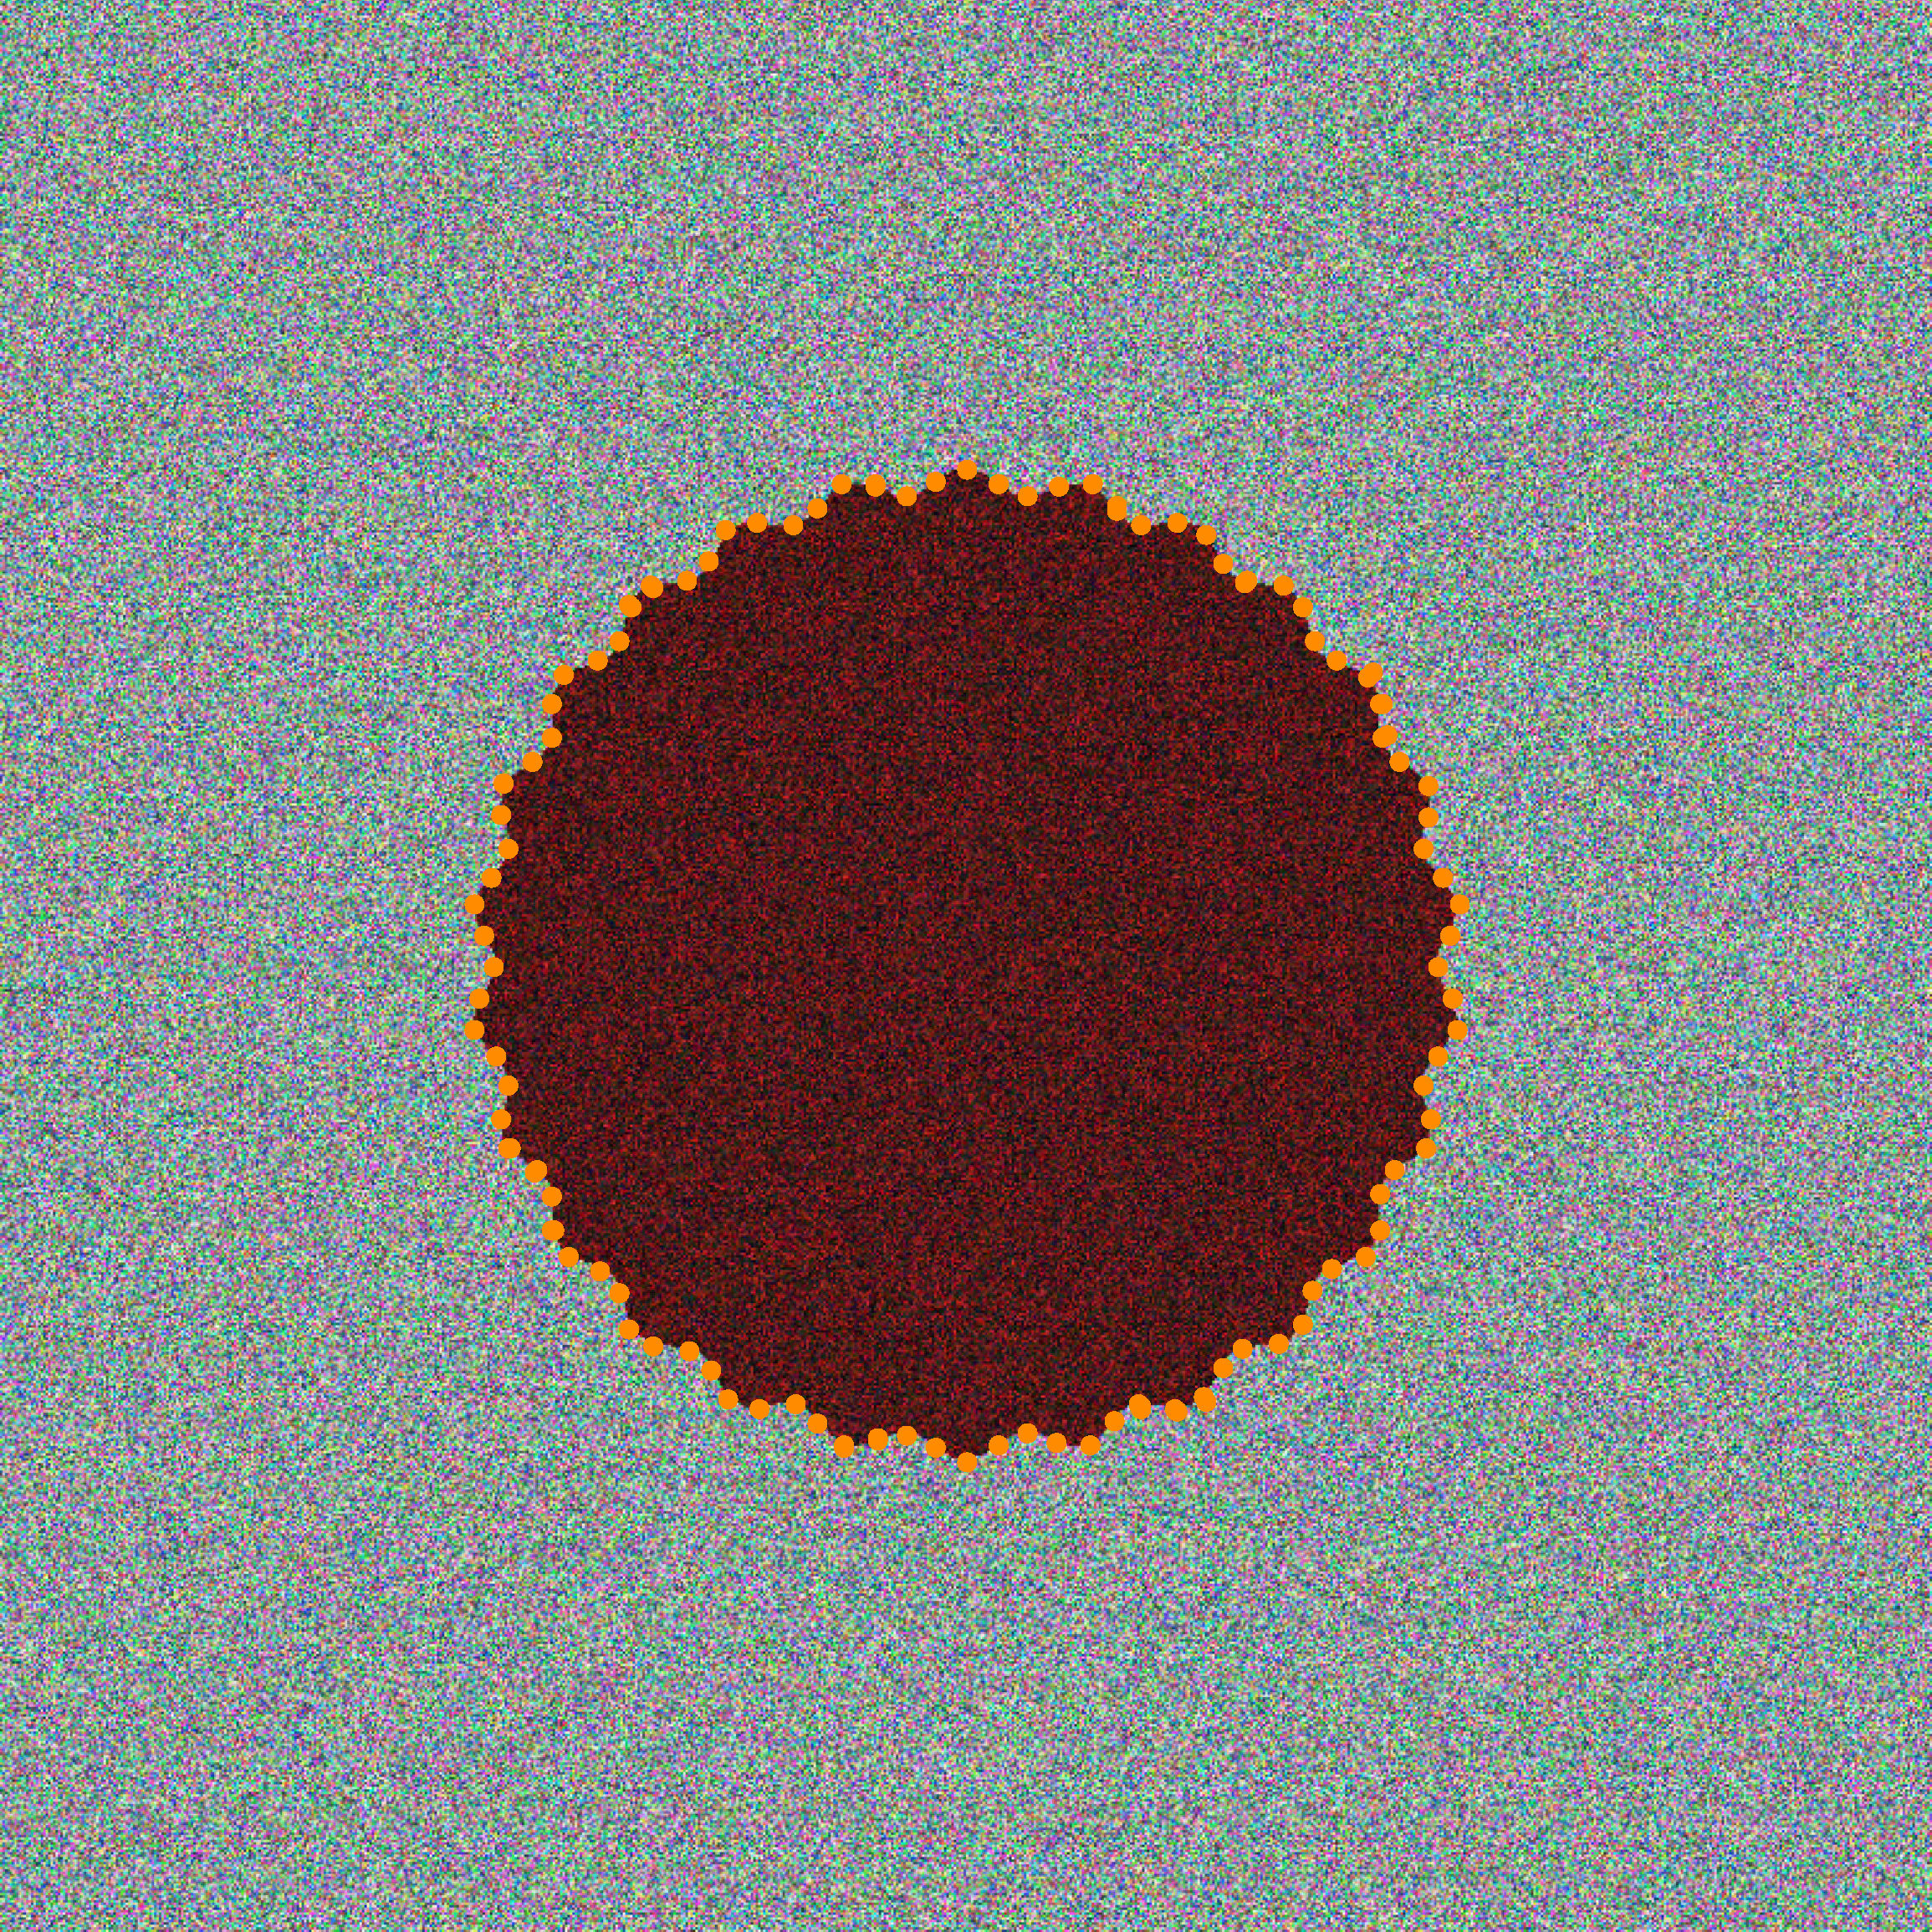
\includegraphics[width=0.26\linewidth]{SimFusionRocRoi01}
     } \\
          \subfloat[S01 image fusion \label{roc_fusion:d}]{%
       \includegraphics[width=0.3\linewidth]{DpbFusionRocRoi01_sc07}
     }
     \subfloat[S02 image fusion\label{roc_fusion:e}]{%
       \includegraphics[width=0.3\linewidth]{DpbFusionRocRoi01_sc10}
     } 
     \caption{Image S-ROC fusion.}
     \label{roc_fusion}
   \end{figure} 
\begin{figure}[hbt]
	\centering
     \subfloat[FLEV image fusion \label{t_roc_fusion:a}]{%
       \includegraphics[width=0.3\linewidth]{FlevFusionRocRoi01_crop_threshold}
     }
     \subfloat[SF image fusion\label{t_roc_fusion:b}]{%
       \includegraphics[width=0.3\linewidth]{SfFusionRocRoi01_crop_threshold}
     }
     \subfloat[SIM image fusion\label{t_roc_fusion:c}]{%
       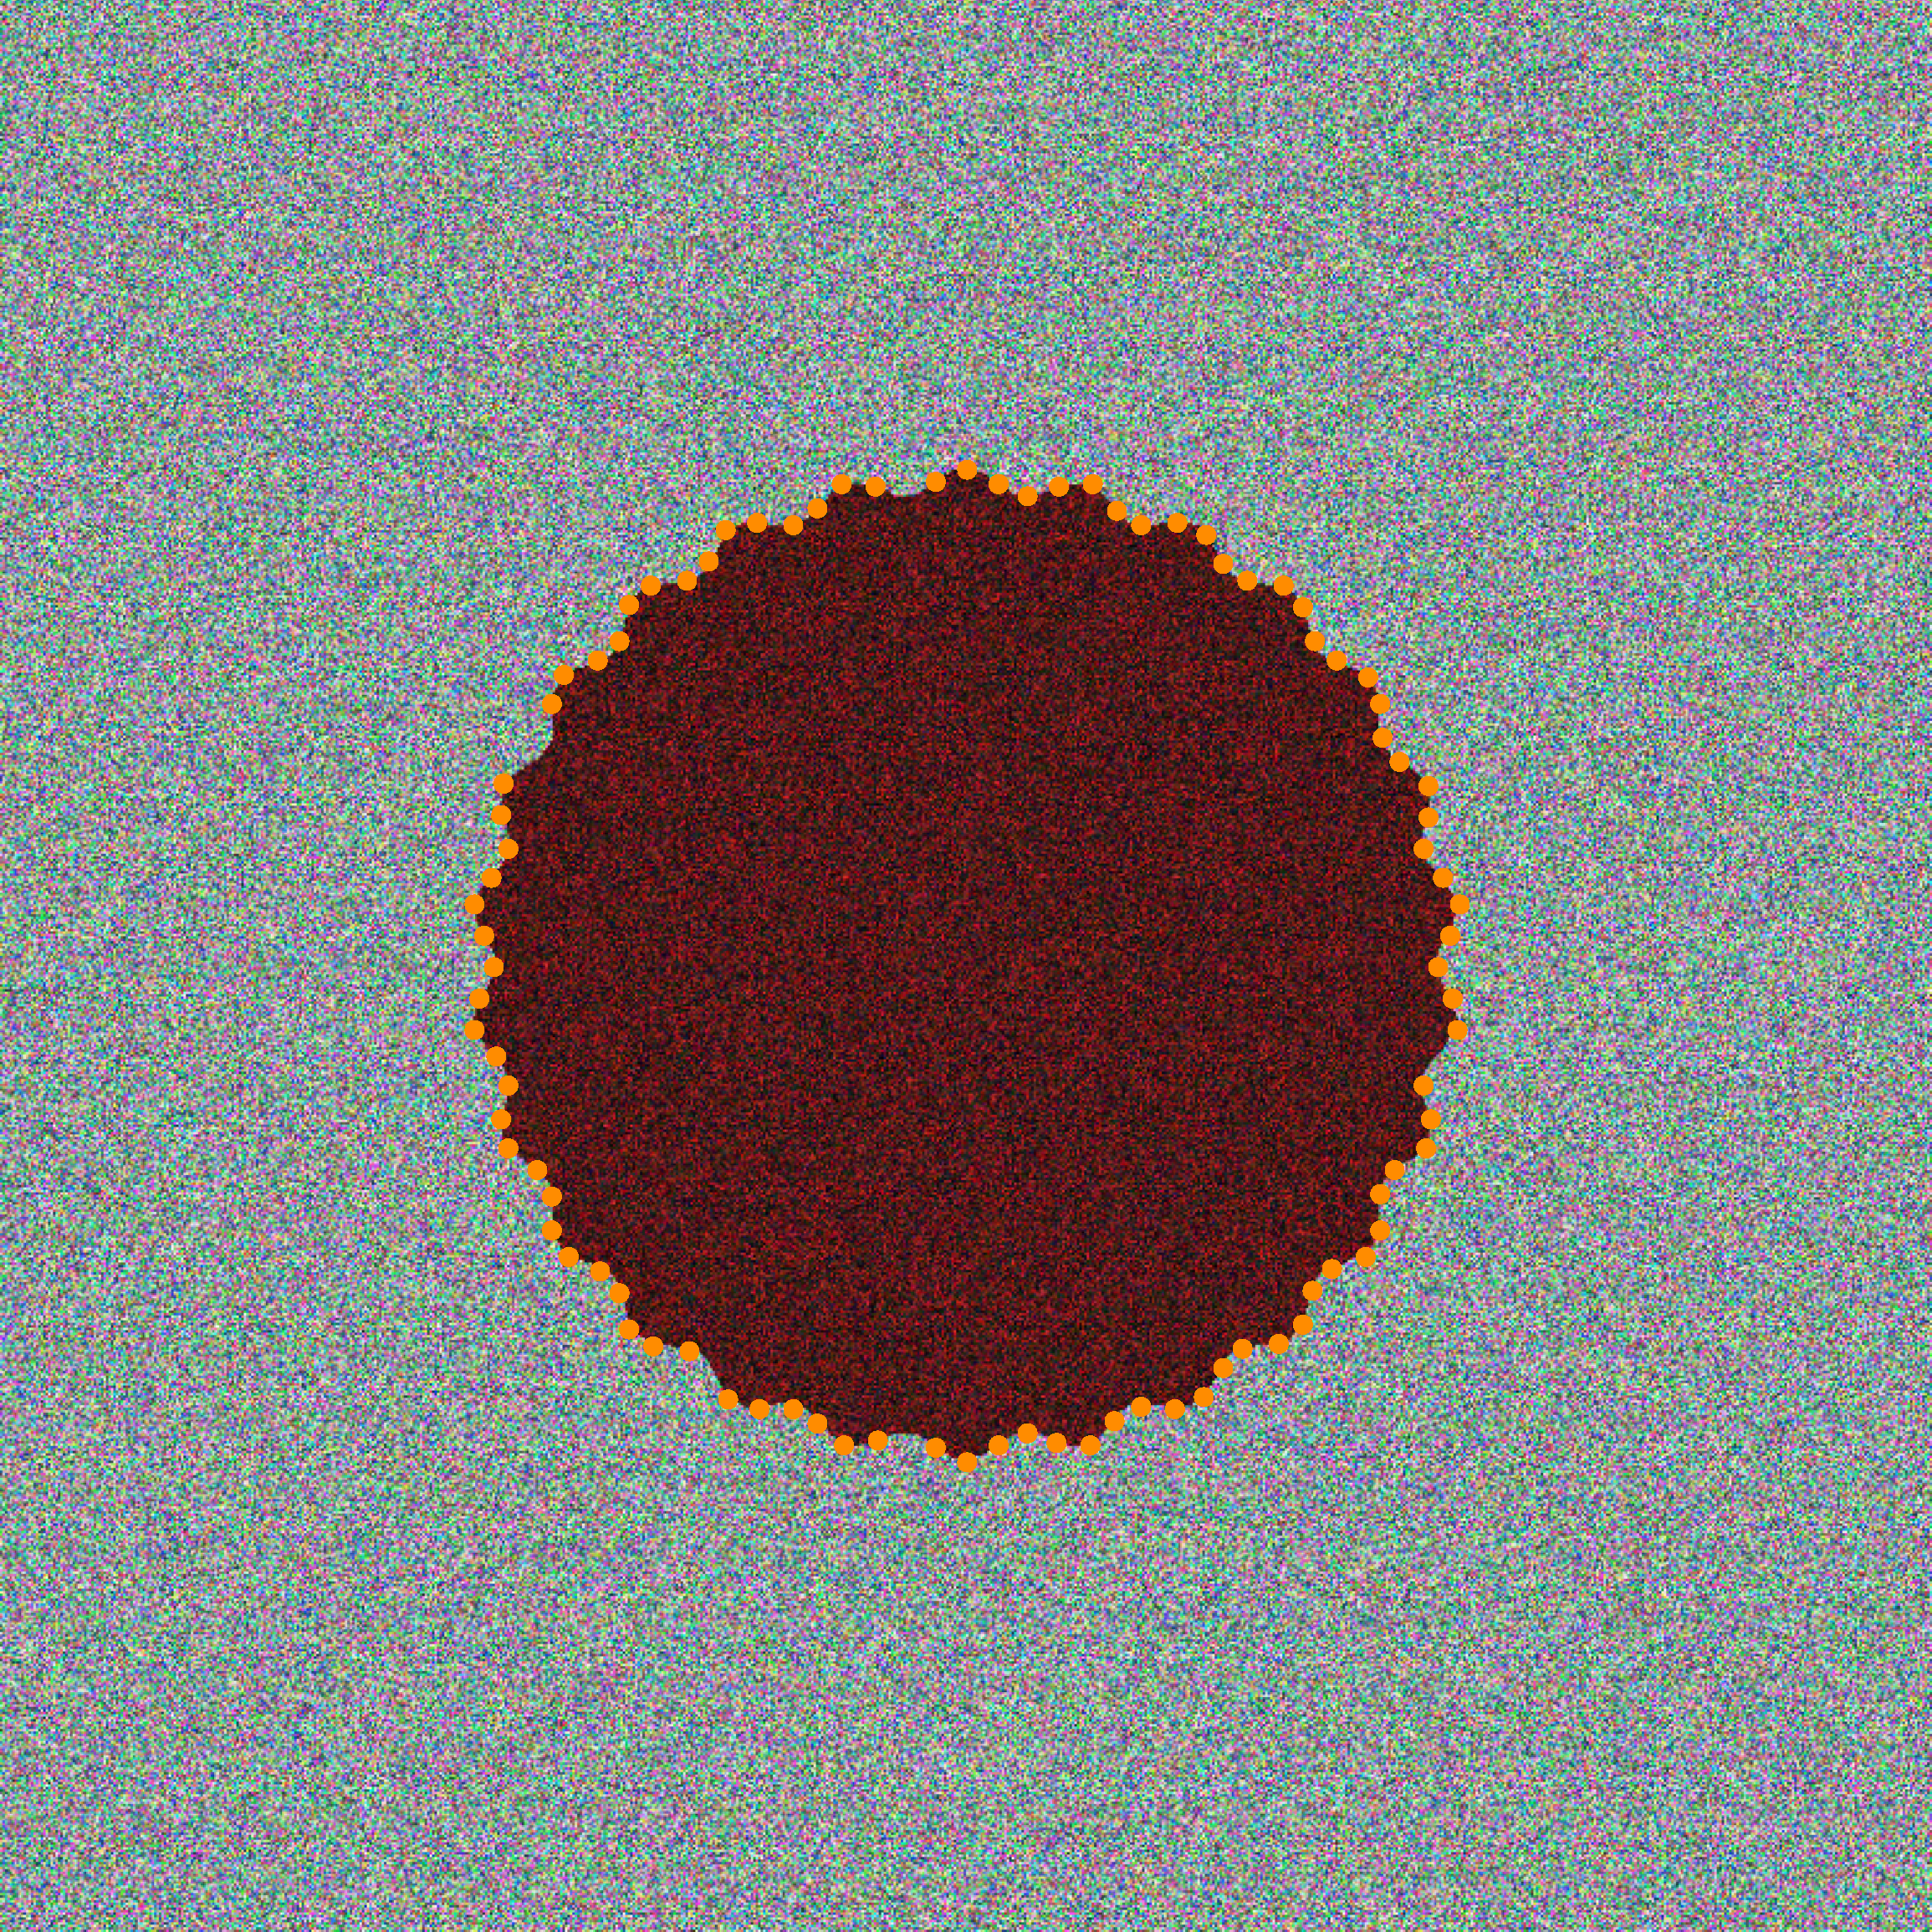
\includegraphics[width=0.26\linewidth]{SimFusionRocRoi01_threshold}
     } \\
          \subfloat[S01 image fusion \label{t_roc_fusion:d}]{%
       \includegraphics[width=0.3\linewidth]{DpbFusionRocRoi01_sc07_threshold}
     }
     \subfloat[S02 image fusion\label{t_roc_fusion:e}]{%
       \includegraphics[width=0.3\linewidth]{DpbFusionRocRoi01_sc10_threshold}
     } 
     \caption{Image $\tau$S-ROC fusion.}
     \label{t_roc_fusion}
   \end{figure}   
\section{Change detection}\label{sec:Change_detection}
We propose a method to change detection in a region of interest (ROI) based on edge detection conform described in this text and Ref~\citet{FusionofEvidencesinIntensitiesChannelsforEdgeDetectioninPolSARImages}. 

The additional idea is to have control of the radial at the uniform region. Therefore, we calculate the log-likelihood function at each point of the radial. After this, we find the mean ($\mu$) and the standard deviation $\sigma$ to define the threshold $\tau=\mu \pm \alpha \sigma$. The constant $\alpha = 0.25$ was chosen empirically. 

We apply the two methodologies to LAA image and the Fig.~\eqref{LA_april_2009_after_before_use_mean_threshold} shows the result. First, the image~\eqref{LA_april_2009_after_before_use_mean_threshold:a} shows the methodology standard and with it we can see the presence of outliers. Second, the image~\eqref{LA_april_2009_after_before_use_mean_threshold:b} shows the methodology with threshold and as this methodology has a good performance to avoid finding edge evidence in the same region. Therefore, we can see that the edge evidences agree with the transition point between two regions. We choose to show the channel HH, however the performance works well for all channels to impact also the edge evidence fusion.  
\begin{figure}[hbt]
	\centering
     \subfloat[Standard methodology \label{LA_april_2009_after_before_use_mean_threshold:a}]{%
       \includegraphics[width=0.35\textwidth]{la_img1_april_2009_ChhRoi01_crop_gray_unless_mean_th}
     }
     \subfloat[Threshold methodology\label{LA_april_2009_after_before_use_mean_threshold:b}]{%
       \includegraphics[width=0.35\linewidth]{la_img1_april_2009_ChhRoi01_crop_gray_with_mean_th}
     }
     \caption{Edge evidence methodologies apply to the LAA (HH intensity channel)}
     \label{LA_april_2009_after_before_use_mean_threshold} 
   \end{figure}

The Fig.~\eqref{LA_GR_images}  shows two coregistered images for the same regions in Los Angeles, California, USA. The Jet Propulsion Laboratory/National Aeronautics and Space Administration (JPL) acquired the images using  the Uninhabited Aerial Vehicle Synthetic Aperture Radar (UAVSAR) with L-band polarimetric multilook. The image~\eqref{LA_GR_images:a} was acquired on April 23, 2009, and the image~\eqref{LA_GR_images:b} was acquired on May 11, 2015. 

The images in Fig~\eqref{LA_april_2009_threshold} show Pauli decomposition in gray-scale overlain     
with edge evidence (Images~\eqref{LA_april_2009_threshold:a} and~\eqref{LA_april_2009_threshold:b}) and edge detected with the information fusion $\tau$S--ROC (Images~\eqref{LA_april_2009_threshold:c} and~\eqref{LA_april_2009_threshold:d}) to the region of interest (ROI). The results shown in this figure were built using methods with uniform control regions.

  \begin{figure}[hbt]
	\centering
     \subfloat[Channel HH edge evidence \label{LA_april_2009_threshold:a}]{%
       \includegraphics[width=0.35\textwidth]{la_img1_april_2009_ChhRoi01_crop_gray_with_mean_th}
     }
     \subfloat[Channel Span edge evidence \label{LA_april_2009_threshold:b}]{%
       \includegraphics[width=0.35\linewidth]{la_img1_april_2009_SpanRoi01_crop_gray_threshold}
     }\\
     \subfloat[S-ROC fusion edge\label{LA_april_2009_threshold:c}]{%
       \includegraphics[width=0.35\linewidth]{la_img1_april_2009_FusionRocRoi01_crop_gray}
     }
     \subfloat[$\tau$S-ROC fusion edge \label{LA_april_2009_threshold:d}]{%
       \includegraphics[width=0.35\linewidth]{la_img1_april_2009_FusionRocRoi01_crop_gray_threshold}
     }
     \caption{Edge evidence and edge detection with uniform region control apply to LAA image} 
     \label{LA_april_2009_threshold} 
   \end{figure}

The images in Fig~\eqref{LA_may_2015_threshold} show Pauli decomposition in gray-scale overlain     
with edge evidence (Images~\eqref{LA_may_2015_threshold:a} and~\eqref{LA_may_2015_threshold:b}) and edge detected with the information fusion (Images~\eqref{LA_may_2015_threshold:c} and~\eqref{LA_may_2015_threshold:d}) to the region of interest (ROI). The results shown in this figure were built using methods with uniform control regions.
  \begin{figure}[hbt]
	\centering
     \subfloat[Channel HH edge evidence  \label{LA_may_2015_threshold:a}]{%
       \includegraphics[width=0.35\textwidth]{la_img1_may_2015_ChhRoi01_crop_gray_threshold}
     }
     \subfloat[Channel Span edge evidence \label{LA_may_2015_threshold:b}]{%
       \includegraphics[width=0.35\linewidth]{la_img1_may_2015_SpanRoi01_crop_gray_threshold}
     }\\
     \subfloat[S-ROC fusion edge \label{LA_may_2015_threshold:c}]{%
       \includegraphics[width=0.35\linewidth]{la_may_2015_FusionRocRoi01_crop_gray}
     }
     \subfloat[$\tau$S-ROC fusion edge \label{LA_may_2015_threshold:d}]{%
       \includegraphics[width=0.35\linewidth]{la_may_2015_FusionRocRoi01_crop_gray_threshold}
     }
     \caption{Edge evidence and edge detection with uniform region control apply to LAM image}
     \label{LA_may_2015_threshold} 
   \end{figure}   

Change detection in multilook polarimetric image SAR (PolSAR) with the methods to detect the edge evidence and the edge using uniform region control works accurately. The S--ROC and the $\tau$S--ROC were applied and shown in the images in Fig~\eqref{LA_april_2009_may_2015_mean_th:a} and  Fig~\eqref{LA_april_2009_may_2015_mean_th:b}.
\begin{figure}[hbt]
	\centering
     \subfloat[Threshold methodology apply in LAA image\label{LA_april_2009_may_2015_mean_th:a}]{%
      % \includegraphics[width=0.35\textwidth]{la_img1_april_2009_ChhRoi01_crop_gray_with_mean_th}
      \includegraphics[width=0.35\textwidth]{la_img1_april_2009_FusionRocRoi01_crop_gray_threshold}
     }
     \subfloat[Threshold methodology apply in LAM image\label{LA_april_2009_may_2015_mean_th:b}]{%
%       \includegraphics[width=0.35\linewidth]{la_img1_may_2015_ChhRoi01_crop_gray_threshold}
       \includegraphics[width=0.35\linewidth]{la_may_2015_FusionRocRoi01_crop_gray_threshold}
     }
     \caption{Change detection in multilook PolSAR image}
     \label{LA_april_2009_may_2015_mean_th} 
   \end{figure}   
%%%%%%%%%%%%%%%%%%%%%%%%%%%%%%%%%%%%%%%%%%
\section{Discussion}\label{sec:Discussion}
In this section, we pointed out and discussed the results obtained in this research:
 
\begin{enumerate}[label=(\roman*)]
%
\item The Bresenham line algorithm was used to extract information from the image. Suppose we define a maximum number of pixels (N) in each radial. Then, the algorithm returns radials with less length than N. Furthermore, the Bresenham algorithm extracts pixels with zero value. When this happens, the pixel is dropped.\label{item:Discuss_01}
%
\item To optimize the log-likelihood reduction it is necessary to calculate the estimated initial parameters ($\mu$, L) to PDF gamma, and  ($\mu$, L, $\rho$, and $\tau$) to PDF ratio of intensities. The initial estimate works better for probability densities function gamma to intensities channels comparability with the probability densities ratio of intensities channels. In this research, we used the BFGS methods to ensure convergence to the maximum of the function log-likelihood reduced.\label{item:Discuss_02}
\item The Hausdorff distance calculated with the methodology presented, see~\eqref{tab:Hausd_dist_channels},  and visual inspection of the image shows the worst performance of the method to edge detection evidence in the HH/VV and VV/HH channels. The PDF using span also shows better measures for Hd distance compatible with the images shown for the Span channel.\label{item:Discuss_03}
%
\item The images in Figs~\eqref{SimRatioRoi01_gray_HHVV_VVHH},~\eqref{FlevRatioRoi01_gray_HHVV_VVHH},~\eqref{SfRatioRoi01_gray_HHVV_VVHH}, and~\eqref{sc_07_RatioRoi01_gray_HHVV_VVHH} show the channels building with the ratio between the intensities channels. We chose this image based on item~\ref{item:Discuss_03}. Furthermore, analyzing the last two image choices, we observe that it is difficult to see regions and features influencing edge evidences detection, as we can confirm in the analysis of the principal coefficients of the PCA method, see Tab\eqref{tab:pca_coeff}.\label{item:Discuss_04}
%
\item The methodology applied in image channels HH/VV and VV/HH shows a similar position to edges evidence detected by images SIM, FLEV, and SF. We can see by visual inspection in Figs~\eqref{sim_ev_intensities_and_ratio:c},~\eqref{sim_ev_intensities_and_ratio:d}, Figs~\eqref{flev_ev_hh_hv_vv:c},~\eqref{flev_ev_hh_hv_vv:d}, and Figs\eqref{sf_ev_hh_hv_vv:c},~\eqref{sf_ev_hh_hv_vv:d}. In Tab~\eqref{tab:Hausd_dist_channels}, we see metric Hd equally applied in this channel's images. In the Santos City image S01 note in Figs~\eqref{sc_07_ev_hh_hv_vv:c}, and~\eqref{sc_07_ev_hh_hv_vv:d} has a difference in edges evidence detected. Furthermore, Tab~\eqref{tab:Hausd_dist_channels} shows the difference between Hd metrics of the images S01 and S02 to the image channels HH/VV and VV/HH. \label{item:Discuss_05}
%
\item Tab~\eqref{tab:pca_coeff} shows that the PCA method recommends the fusion of the intensities or span channels, except image S02, so we use this channel to build the fusion methods $\tau$S--ROC. 
Analyzing the table~\eqref{tab:fusion_Hausd_dist_channels}, we notice that the proposed method $\tau$S--ROC performs better when considering the metric Hd because it reached the lowest value in most tests performed with the images. Again the exception was image S02. 
We can affirm  S02 is the unique image in Fig~\eqref{GR_images} where the channel's information using the pdf ratio of intensities contributes to the fusion method $\tau$S--ROC.  
 \label{item:Discuss_06}
%
\item The visual inspection of the Figs~\eqref{roc_fusion} and~\eqref{t_roc_fusion} shows the advantage that the proposed method to the information fusion $\tau$S--ROC has in recognizing and discarding outliers with relation to the S--ROC. The quality of this information captured with the $\tau$S--ROC method can be improved by inserting the optical channels image in the fusion process. Furthermore, in PolSAR image, we can insert other channels using physical or empirical PDF.
 \label{item:Discuss_07}
% 
\item The methods proposed to obtain the edge evidences and the edges using the information fusion (S--ROC, and $\tau$S--ROC)  work well when applied to images obtained by different sensors. The remainder of FLEV and SF was obtained with AIRSAR sensor, S01, and S02 were obtained with OrbiSAR-2 sensor, and finally, the LAA and LAM were obtained with UAVSAR sensor. \label{item:Discuss_08}
\item  The Fig~\eqref{LA_april_2009_after_before_use_mean_threshold} shows the methodology to edge evidence applied to LAA in image~\eqref{LA_april_2009_after_before_use_mean_threshold:a} and the threshold methodology to recognize the same regions in ~\eqref{LA_april_2009_after_before_use_mean_threshold:b}. In this case, the methodology was applied in HH channel. We can verify that the methodology with the threshold proposed can eliminate the point detected in the same region. We highlight in the last figure that the methodology detected accurate edges evidences. \label{item:Discuss_9}
\item Fig~\eqref{LA_april_2009_threshold} and~\eqref{LA_may_2015_threshold} show the results of the threshold methodology to detect edge evidence (HH, and Span channel) and detect edge (E--ROC and TE--ROC). \label{item:Discuss_10}
\item The previous item~\ref{item:Discuss_10} motivated us to check the change detection in two images of Los Angeles taken from the same region at different times. The result is shown in Fig~\eqref{LA_april_2009_may_2015_mean_th}. The visual inspection of Fig~\eqref{LA_april_2009_may_2015_mean_th:a}  (LAA image) and the Fig~~\eqref{LA_april_2009_may_2015_mean_th:b} (LAM image) shows the capacity of the methods obtain change detect to the UAVSAR PolSAR image. \label{item:Discuss_11}

\item The figures show the behavior of the method for detecting uniform regions in the LAA and LAM images; by performing a visual inspection, we can notice that the method has the ability to detect changes between images of the same region captured at different times.  \label{item:Discuss_12}

\end{enumerate}

\section{Conclusion}\label{sec:Conclusion}

%%%%%%%%%%%%%%%%%%%%%%%%%%%%%%%%%%%%%%%%%%
\authorcontributions{For research articles with several authors, a short paragraph specifying their individual contributions must be provided. The following statements should be used ``Conceptualization, X.X. and Y.Y.; methodology, X.X.; software, X.X.; validation, X.X., Y.Y. and Z.Z.; formal analysis, X.X.; investigation, X.X.; resources, X.X.; data curation, X.X.; writing---original draft preparation, X.X.; writing---review and editing, X.X.; visualization, X.X.; supervision, X.X.; project administration, X.X.; funding acquisition, Y.Y. All authors have read and agreed to the published version of the manuscript.'', please turn to the  \href{http://img.mdpi.org/data/contributor-role-instruction.pdf}{CRediT taxonomy} for the term explanation. Authorship must be limited to those who have contributed substantially to the work~reported.}

\funding{This research was funded by Conselho Nacional de Desenvolvimento Científico e Tecnológico -- CNPq, grant number 200725/2022-0.}
%Please add: ``This research received no external funding'' or ``This research was funded by NAME OF FUNDER grant number XXX.'' and  and ``The APC was funded by XXX''. Check carefully that the details given are accurate and use the standard spelling of funding agency names at \url{https://search.crossref.org/funding}, any errors may affect your future funding.}


\dataavailability{In this section, please provide details regarding where data supporting reported results can be found, including links to publicly archived datasets analyzed or generated during the study. Please refer to suggested Data Availability Statements in section ``MDPI Research Data Policies'' at \url{https://www.mdpi.com/ethics}. If the study did not report any data, you might add ``Not applicable'' here.} 

\acknowledgments{In this section you can acknowledge any support given which is not covered by the author contribution or funding sections. This may include administrative and technical support, or donations in kind (e.g., materials used for experiments).}

\conflictsofinterest{Declare conflicts of interest or state ``The authors declare no conflict of interest.'' Authors must identify and declare any personal circumstances or interest that may be perceived as inappropriately influencing the representation or interpretation of reported research results. Any role of the funders in the design of the study; in the collection, analyses or interpretation of data; in the writing of the manuscript; or in the decision to publish the results must be declared in this section. If there is no role, please state ``The funders had no role in the design of the study; in the collection, analyses, or interpretation of data; in the writing of the manuscript; or in the decision to publish the~results''.} 

%%%%%%%%%%%%%%%%%%%%%%%%%%%%%%%%%%%%%%%%%%
%% Optional

%% Only for journal Encyclopedia
%\entrylink{The Link to this entry published on the encyclopedia platform.}

\abbreviations{Abbreviations}{
The following abbreviations are used in this manuscript:\\

\noindent 
\begin{tabular}{@{}ll}
PDF & Probability Density Function\\
GR & Ground Reference\\
SAR & Synthetic Aperture Radar\\
PolSAR & Polarimetric Synthetic Aperture Radar\\
AIRSAR & Airborne Synthetic Aperture Rada\\
OrbiSAR-2 & Orbital SAR \\ 
UAVSAR & Uninhabited Aerial Vehicle Synthetic Aperture Radar\\
SIM & Flower Simulated Image \\
FLEV& Flevoland Image\\
SF  & San Francisco Image\\
S01 & Sub-scene 01 of Santos City\\
S02 & Sub-scene 02 of Santos City\\
LAA & Los Angeles Image on April 2009\\
LAM & Los Angeles Image on May 2015\\
ROI & Region Of Interest\\
MLE & Maximum Likelihood Estimator\\
BFGS & Broyden-Fletcher-Goldfarb-Shanno \\
GenSA & Generalized Simulated Annealing \\
S--ROC & Statistic Receiver Operating Characteristic\\
$\tau$S--ROC &Statistic Receiver Operating Characteristic with a threshold \\
PCA & Principal Components Analysis\\
Hd & Hausdorff Distance \\
\end{tabular}
}
 %%%%%%%%%%%%%%%%%%%%%%%%%%%%%%%%%%%%%%%%%%
%% Optional
\appendixtitles{yes} % Leave argument "no" if all appendix headings stay EMPTY (then no dot is printed after "Appendix A"). If the appendix sections contain a heading then change the argument to "yes".
\appendixstart
\appendix

%%%%%%%%%%%%%%%%%%%%%%%%%%%%%%%%%%%%%%%%%%
\begin{adjustwidth}{-\extralength}{0cm}
%\printendnotes[custom] % Un-comment to print a list of endnotes

\reftitle{References}

% Please provide either the correct journal abbreviation (e.g. according to the “List of Title Word Abbreviations” http://www.issn.org/services/online-services/access-to-the-ltwa/) or the full name of the journal.
% Citations and References in Supplementary files are permitted provided that they also appear in the reference list here. 

%=====================================
% References, variant A: external bibliography
%=====================================
\bibliography{references} 
 % If authors have biography, please use the format below
%\section*{Short Biography of Authors}
%\bio
%{\raisebox{-0.35cm}{\includegraphics[width=3.5cm,height=5.3cm,clip,keepaspectratio]{Definitions/author1.pdf}}}
%{\textbf{Firstname Lastname} Biography of first author}
%
%\bio
%{\raisebox{-0.35cm}{\includegraphics[width=3.5cm,height=5.3cm,clip,keepaspectratio]{Definitions/author2.jpg}}}
%{\textbf{Firstname Lastname} Biography of second author}

% For the MDPI journals use author-date citation, please follow the formatting guidelines on http://www.mdpi.com/authors/references
% To cite two works by the same author: \citeauthor{ref-journal-1a} (\citeyear{ref-journal-1a}, \citeyear{ref-journal-1b}). This produces: Whittaker (1967, 1975)
% To cite two works by the same author with specific pages: \citeauthor{ref-journal-3a} (\citeyear{ref-journal-3a}, p. 328; \citeyear{ref-journal-3b}, p.475). This produces: Wong (1999, p. 328; 2000, p. 475)

%%%%%%%%%%%%%%%%%%%%%%%%%%%%%%%%%%%%%%%%%%
%% for journal Sci
%\reviewreports{\\
%Reviewer 1 comments and authors’ response\\
%Reviewer 2 comments and authors’ response\\
%Reviewer 3 comments and authors’ response
%}
%%%%%%%%%%%%%%%%%%%%%%%%%%%%%%%%%%%%%%%%%%
\end{adjustwidth}
\end{document}

